\documentclass[twocolumn,showpacs,preprintnumbers,nofootinbib,prd,
superscriptaddress,10pt]{revtex4-2}

\usepackage{amsmath,amssymb}
\usepackage{amsfonts}
\usepackage{mathtools}
\usepackage[normalem]{ulem}
\usepackage{textcomp}
\usepackage{enumitem}
\usepackage{bm}
\usepackage{bbm}
\usepackage{afterpage}
%\usepackage{float}
\usepackage{graphicx}
\usepackage{subcaption}
\graphicspath{{img/}} %setting img path

\usepackage{tabularx, longtable, makecell}
\usepackage{multirow}
\usepackage{arydshln}

\usepackage{tensor}
\usepackage{layouts}
\usepackage[usenames,dvipsnames]{xcolor}
\usepackage[utf8]{inputenc}
\usepackage{algorithm}
\usepackage{algpseudocode}
\usepackage{rotating}
\usepackage[bookmarks]{hyperref}
%\usepackage{ragged2e}
\usepackage{blindtext}
\usepackage{graphicx}
\usepackage{siunitx}
	\sisetup{output-decimal-marker={.}}
	
	%some math symbols
\newcommand{\R}{\mathbb{R}}
\newcommand{\N}{\mathbb{N}}
\DeclareMathOperator{\sign}{sign}
\renewcommand{\d}[1]{\ensuremath{\operatorname{d}\!{#1}}}
\newcommand{\dvol}[2]{\ensuremath{\operatorname{d}^{#2}\!{#1}}}
%argmin and argmax
\DeclareMathOperator*{\argmax}{arg\,max}
\DeclareMathOperator*{\argmin}{arg\,min}

\newcommand{\scalar}[2]{\langle #1|#2 \rangle}
\newcommand{\scalarnonorm}[2]{\langle #1|#2 \rangle_{\text{not normalized}}}
\newcommand{\rescalar}[2]{( #1|#2 )}
\newcommand{\imscalar}[2]{[ #1|#2 ]}


% comments command
\newcommand{\stefano}[1]{{\textcolor{blue}{\texttt{SS: #1}} }}
\newcommand{\sarah}[1]{{\textcolor{red}{\texttt{SC: #1}} }}
\newcommand{\bhooshan}[1]{{\textcolor{cyan}{\texttt{BG: #1}} }}
\newcommand{\oldnewtxt}[2]{\sout{#1}\textcolor{red}{#2}}


\begin{document}

	%%%%%%%%%%%%%%%%%%%%%%%%%%%%%%%%% ABSTRACT
\begin{abstract}
	We introduce a novel method to generate a bank of gravitational-waveform templates of binary black hole (BBH) coalescences for matched-filter searches in LIGO, Virgo and Kagra data. Unlike the standard approach, our method relies on a numerical metric approximation of the distance between templates, which makes the template placement orders of magnitude faster than with existing techniques.
	Our method applies to a variety of different manifolds of signals and is particularly suitable for covering high dimensional spaces, such as those associated with precessing and/or eccentric waveforms.
	We compare our method with the state-of-the-art stochastic placement code and we find that our code slightly overcovers the space, while achieving similar efficiency in recovering signals. To demonstrate the capabilities of our code, we generate a precessing bank, an intermediate mass black hole bank with higher-order modes, and an eccentric bank, and show that they cover the space in a satisfactory way.
	Our publicly released code \texttt{mbank} will enable searches of high dimensional regions of BBH signal space, hitherto unfeasible due to the prohibitive cost of bank generation.
\end{abstract}
	
	%%%%%%%%%%%%%%%%%%%%%%%%%%%%%%%%% TITLE
	\title{Metric template placement for high dimensional regions of compact binary mergers}
	\author{Stefano \surname{Schmidt}}
		\email{s.schmidt@uu.nl}
        \affiliation{Nikhef, Science Park 105, 1098 XG, Amsterdam, The Netherlands}
        \affiliation{Institute for Gravitational and Subatomic Physics (GRASP),
Utrecht University, Princetonplein 1, 3584 CC Utrecht, The Netherlands}

	\author{Bhooshan \surname{Gadre}}
        \affiliation{Institute for Gravitational and Subatomic Physics (GRASP),
Utrecht University, Princetonplein 1, 3584 CC Utrecht, The Netherlands}
        
        %
	\author{Sarah \surname{Caudill}}
%        \affiliation{Nikhef, Science Park 105, 1098 XG, Amsterdam, The Netherlands}
%        \affiliation{Institute for Gravitational and Subatomic Physics (GRASP),
%Utrecht University, Princetonplein 1, 3584 CC Utrecht, The Netherlands}
		\affiliation{Department of Physics, University of Massachusetts, Dartmouth, MA 02747, USA}
		\affiliation{Center for Scientific Computing and Visualization Research, University of Massachusetts, Dartmouth, MA 02747, USA}
	\maketitle

	%\tableofcontents

	%%%%%%%%%%%%%%%%%%%%%%%%%%%%%%%%% BODY 
\section{Introduction}

As gravitational-wave (GW) astronomy enters a mature state, the accessible parameter space of binary black hole (BBH) mergers in LIGO \cite{LIGOScientific:2014pky} and Virgo \cite{VIRGO:2014yos} data continues to grow. Besides standard aligned-spin GW searches for stellar-mass BBH mergers \cite{GWTC-1,GWTC-2,GWTC-2.1, GWTC-3}, there are GW searches targeting the parameter space of sub-solar mass black holes (BH) \cite{SSM_O2, SSM_O3a, PhysRevD.106.023024, Nitz:2021mzz}, primordial BHs \cite{PBH}, eccentric binaries \cite{PhysRevD.102.043005, PhysRevD.104.104016, Nitz:2019spj} and intermediate-mass BHs (IMBH) \cite{IMBH_O2, IMBH_O3, Chandra:2022ixv}. Moreover, there is a growing interest in GW searches for more complex binaries, such as those with precession \cite{PhysRevD.89.024010, PhysRevD.97.023004, PhysRevD.102.041302, Indik:2016qky, Harry:2016ijz}, eccentricity \cite{LIGOScientific:2019dag, Ramos-Buades:2020eju, Wang:2021qsu, Nitz:2021mzz} or higher-order mode (HMs) content~\cite{CalderonBustillo:2015lrt, PhysRevD.97.023004, Chandra_hom, 2021PhRvD.103b4042M}.

GW searches for signals from compact binary mergers traditionally utilize the method of matched-filtering with a template bank of model waveforms~\cite{Sathyaprakash:1991mt, Dhurandhar:1992mw, Owen:1998dk, Allen:2005fk, Babak:2006ty, Cokelaer:2007mv}. Accurate template banks that cover the parameter space of interest can be computationally expensive to create, but are crucial for ensuring sensitivity of state-of-the-art searches.

One widely used approach to bank generation - the {\it stochastic} method \cite{Harry:2009ea, PhysRevD.80.104014, Ajith:2012mn} - consists of randomly scattering templates in a defined parameter space with a rejection technique \cite{DalCanton:2017ala, Mukherjee:2018yra, Indik:2016qky, Lenon:2021zac}. A proposed template is included in the bank only if its distance (or {\it mismatch}) with all the proposed templates in the bank is larger than the user-defined threshold.
While this method is proven to work in many cases, it is computationally demanding, since it requires the generation of a huge number of template waveforms and expensive match calculations.
With the ever-growing hyper-volume of parameter space for BBH searches, current approaches will quickly become computationally intractable.

Revitalizing a pioneering line of research in bank generation \cite{owen_metric, Messenger:2008ta, Prix:2007ks, Brown:2012qf, Keppel:2013uma}, there has been recently an increasing attention on {\it metric template placement} \cite{Roy:2017oul, 2018cosp...42E2899R, Coogan:2022qxs, Hanna:2022zpk}.
Such methods rely on approximating the distance (or match) between two waveforms with a bilinear form. Despite being approximate, they allow for a faster template placing that may overcome some of the major limitations of the standard stochastic placement algorithm.

In this work, we develop a novel approach to template placing based on the metric approximation of the mismatch.
Our method is specifically designed for dealing with high-dimensional ($>$ 4D) template banks of GWs signals, making it particularly suitable for precessing or eccentric searches.
Our method is implemented in an open-source, production-ready, python package \texttt{mbank}, available on GitHub\footnote{
It is available at the repository \href{https://github.com/stefanoschmidt1995/mbank}{stefanoschmidt1995/mbank}.}
and on the PyPI repository\footnote{
In the PyPI repository, the package is distributed under the name \texttt{\href{https://pypi.org/project/gw-mbank/}{gw-mbank}}.
}.

%Compared to other codes, \texttt{mbank} is designed to be:
%\begin{itemize}
%	\item Orders of magnitude faster than the state-of-the-art
%	\item Suitable to cover a high dimensional parameter space
%	\item Close to provide optimal coverage
%\end{itemize}

The rest of this paper is devoted to the presentation and description of our methods and package.
In Sec.~\ref{sec:methods} we present the details of the bank generation algorithm.
In Sec.~\ref{sec:validation} we assess the accuracy of the metric approximation and of the template placing methods and also compare our method with the widely-used stochastic placement code \texttt{sbank} \cite{Ajith:2012mn}.
To demonstrate the capabilities of \texttt{mbank}, in Sec.~\ref{sec:bank_generation}, we present three large banks covering ``exotic" regions of parameter space: a precessing bank, an IMBH bank with higher-order modes and an eccentric bank.
Finally, in Sec.~\ref{sec:conclusion} we conclude with some remarks on future prospects.

	%%%%%%%%%%%%%%%%%%%%%%%%%%%%%%%%%
\section{Methods} \label{sec:methods}

When searching for a BBH signal in GW data, it is customary to use a frequentist detection statistic~\cite{Creighton_book, Maggiore:2007ulw, Harry:2016ijz, PhysRevD.97.023004}.
We model the detector output $s(t)$ to be composed of {\it Gaussian} noise $n(t)$ and possibly a known GW signal $h(t)$.
Given some observed data $d(t)$, the detection statistic $\Lambda$ is then a measure of the log probability ratio between the signal hypothesis $s = n+h$ and the noise hypothesis $s = n$:
\begin{equation}\label{eq:LL}
	\Lambda(\theta) = \log\frac{p(s = n+h(\theta)|d)}{p(s = n|d)}
\end{equation}
where a signal model is parameterized by a vector of parameters $\theta$, which represents a GW signal $h(t;\theta)$.
For any given observation time, a search aims to maximize the detection statistics with respect to $\theta$.
The exact expressions of $p(s = n+h(\theta)|d)$ and $p(s = n|d)$ are obtained under the assumption of stationary Gaussian noise and  depend on the quantities $\scalar{s}{h}$ and $\scalar{h}{h}$, where $\scalar{\cdot}{\cdot}$ is a noise-weighted scalar product described in more detail in Sec.~\ref{sec:metric}.

A generic eccentric BBH signal detected by LIGO or Virgo will be characterized by 17 quantities \cite{Sathyaprakash_2009}, grouped into \textit{intrinsic} and \textit{extrinsic} parameters.
The twelve intrinsic parameters needed to fully characterize the source consist of: two BH masses ($m_1$, $m_2$), two 3-dimensional spins ($\mathbf{s}_1$, $\mathbf{s}_2$), the inclination angle $\iota$, the reference phase $\phi$, the eccentricity $e$ of the orbit and the mean periastron anomaly $a$.
The five extrinsic parameters characterize the position of the source with respect to the observer: sky location (two angles: right ascension and declination), luminosity distance $D$, polarization angle $\Psi$ and the time of arrival of the signal.

One is able to maximize $\Lambda(\theta)$ analytically over the extrinsic parameters and, depending on the scope of the search, over many of the intrinsic parameters\footnote{
In the case of a non-precessing BBH, where we neglect the higher-order modes, the parameter space to search by brute force has only 4 dimensions (two masses and the two z-components of the spins).
}.
For the other quantities, a brute force approach is required, where $\Lambda(\theta)$ is evaluated on a large set of values of $\theta$, called a {\it template bank} \cite{PhysRevD.77.104017, Mukherjee:2018yra}.
A GW search filters the data with all the templates of a bank and computes the detection statistic for template as a function of time. This is the process of {\it matched filtering}, implemented by several pipelines to successfully search for GW signals \cite{Privitera:2013xza, Usman:2015kfa, Capano:2016dsf, PhysRevD.95.042001, gstlal_paper2, Aubin:2020goo, Chu:2020pjv}.

It is useful, to think of the BBH parameter space as a D-dimensional manifold $\mathcal{B}_D$, embedded in a large 12 dimensional manifold $\mathcal{B}$. Each point of the manifold corresponds to a GW signal. The number of dimensions $D$ depends on the BBH variables under consideration.
As the parameters that do not enter the interesting space can be freely neglected (i.e. set to $0$ or to a meaningful default value), the manifold $\mathcal{B}_D$ is effectively a lower dimensional {\it projection} of the full manifold $\mathcal{B}$.

%Placing templates on $\mathcal{B}_D$ is a highly non-trivial task, as one has to struggle to ensure a good coverage (and avoid missing any signal) while keeping a low number of templates (and save computational power).
%Throughtout the years many different techniques have been devised to achieve such goal.
%
To place templates on $\mathcal{B}_D$, it is standard to equip the manifold with a distance (called {\it mismatch}) and then place templates so that: (i) they cover all the manifold and (ii) their mutual distance is as close as possible to a target distance.
A template bank meeting the two requirement is said to provide a good {\it coverage} of the space.
Building on this, we develop a novel approach to template placing in three (plus one) steps:

\begin{enumerate}
	\item Construction of a metric approximation of the match between templates. This makes $\mathcal{B}_D$ a Riemannian manifold.
	\item Creation of a tiling (cover) for the manifold. In each tile the metric is assumed to be constant.
	\item \textit{(Optional)} Training of a normalizing flow model to interpolate the metric within each tile and sample from the manifold. 
	\item Placing the templates according to the tiling.
\end{enumerate}
Although this results in template placing that is only approximately optimal, our method is several orders of magnitude faster than the standard stochastic approach, as it avoids the generation of a large number of waveforms.
The rest of this section details the steps above.

\subsection{The metric} \label{sec:metric}

The metric distance on the manifold of templates $\mathcal{B}_D$ provides a a fast-to-compute approximation to the {\it mismatch} between templates. We now derive an explicit expression for the metric in terms of the waveform and its gradients.

Under the assumption of Gaussian noise \cite{Creighton_book}, it is natural to introduce a complex \textit{scalar product}\footnote{
Technically, this is a scalar product on the $L^2$ space of the waveforms $h$.}
$\scalar{\cdot}{\cdot}$ between two templates $h(\theta_1)$ and $h(\theta_2)$, evaluated at different points:

\begin{equation} \label{eq:scalar_product}
	\scalar{h(\theta_1)}{h(\theta_2)} = 4 \int_{0}^{\infty} \d{f} \frac{\tilde{h}^*(f;\theta_1) \tilde{h}(f;\theta_2)}{S_n(f)}
\end{equation}
where $\tilde{h}(f; \theta)$ denotes the frequency-domain template, used to filter the data, evaluated at the point $\theta$ on the manifold.

A template $h(\theta)$ can be normalized using the scalar product above:
\begin{equation} \label{eq:normalization}
	\hat{h}(\theta) = \frac{h(\theta)}{\scalar{h(\theta)}{h(\theta)}}.
\end{equation}

For non-precessing circular BBHs, the two polarization are related by the symmetry relation ${\tilde{h}_+ = i \, \tilde{h}_\times}$ and the template takes a simple expression in terms of the two polarizations: ${\tilde{h}(f; \theta) \propto \tilde{h}_+(f; \theta)}$.
For a more general case, the data needs to be filtered with a more complicated template, which takes into account the additional information brought by the cross polarization.
In this work however, we neglect this fact and we will always approximate the template $\tilde{h}$ with just the plus polarization: ${\tilde{h}(f; \theta) \propto \tilde{h}_+(f; \theta)}$.
\stefano{Here I would be a bit uncorfortable defending the need for this approximation}

%We can use the scalar product to define the sought for distance between signals.
We define the overlap $\mathcal{O}(\theta_1,\theta_2, t)$ between normalized templates as:
\begin{align}\label{eq:overlap}
	\mathcal{O}(\theta_1,\theta_2, t) &= \left\lvert \int\limits_{0}^{+\infty} \d{f} \frac{\tilde{\hat{h}}^*(f;\theta_1)\tilde{\hat{h}}(f;\theta_2) e^{i2\pi ft}}{S_n(f)} \right\rvert \nonumber\\
	&= \lvert \scalar{\hat{h}(\theta_1)}{\hat{h}(\theta_2)e^{i 2\pi ft}} \rvert
\end{align}
where $\hat{h}(\theta)e^{i 2\pi ft}$ is the waveform $\hat{h}(\theta)$ translated by a constant time $t$ and $\lvert \cdot \rvert$ denotes the absolute value of a complex number.

We can use the overlap compute the scalar product between $h(\theta_1)$ and $h(\theta_2)$, maximized over a constant time shift between the two. This is defined as the {\it match}:
\begin{equation}\label{eq:match}
	\mathcal{M}&(\theta_1,\theta_2) = \max_t \mathcal{O}(\theta_1,\theta_2, t). \\
	%&= \max_t \sqrt{ \rescalar{\hat{h}(\theta_1)}{\hat{h}(\theta_2)e^{i 2\pi ft}}^2 + \imscalar{\hat{h}(\theta_1)}{\hat{h}(\theta_2)e^{i2\pi ft}}^2 }  \nonumber 
\end{equation}
%
which takes values in the range $[0,1]$. Trivially $\mathcal{M}(\theta,\theta) = 1$.

We are now ready to define a {\it distance} $d(\theta_1,\theta_2)$ \footnote{
From a strict geometrical point of view, this is not a distance since it does not satisfy triangular inequality. However, this does not affect its effectiveness in measuring the ``dissimilarity" between two waveforms and it will be used regardless.}
on the D-manifold $\mathcal{B}_D$:
\begin{align}\label{eq:distance}
	d(\theta_1,\theta_2) \vcentcolon= \sqrt{1 - \mathcal{M}(\theta_1,\theta_2)}
\end{align}
The quantity $1-\mathcal{M}$ above is also called {\it mismatch}.

To construct the metric approximation of the distance Eq.~\eqref{eq:distance}, we replace the distance with a bilinear form in the neighborhood of any point $\theta$. Such bilinear form is represented by a $D\times D$ matrix $M_{ij}(\theta)$ such that\footnote{
In this expression and everywhere else, we assume Einstein summation convention for the vector product.}:
\begin{align}\label{eq:metric_definition}
	d^2(\theta_1,\theta_2) = 1 - \mathcal{M}(\theta_1,\theta_2) \simeq M_{ij}(\theta) \Delta\theta_i \Delta\theta_j
\end{align}
where $\Delta\theta = \theta_1-\theta_2$ is a D-dimensional vector \cite{owen_metric}.
It is worth noting that, like any expansion, Eq.~\eqref{eq:metric_definition} is guaranteed to be accurate only in the limit of small $||\Delta\theta||$\footnote{Here $||\cdot||$ is the usual Euclidean $L^2$ norm.}.
%For $||\Delta\theta|| \gtrsim 1$ the metric approximation may lose its predictivity power and the validity of the approximation needs to be checked in every situation.

Of course, there is not a ``true" expression for the matrix $M_{ij}(\theta)$, but its value may depend on the application and on the range of validity of the approximation.
A fair guess for the tensor field $M_{ij}(\theta)$ can be done through an optimization problem where we minimize the discrepancy between the metric distance Eq.~\eqref{eq:metric_definition} and the actual distance Eq.~\eqref{eq:distance}.
The disagreement between the two expressions around a point $\theta$ can be encoded into a {\it loss function}, which depends on the values of the matrix elements $M^\prime_{ij}$:
\begin{equation} \label{eq:loss_function}
	\mathcal{L}_\theta(M^\prime_{ij}) = \hspace{-4em} \int\limits_{\hspace{3em}\{d(\theta,\theta^\prime) < d_\mathrm{target}\}} \hspace{-3.8em}
		\dvol{\theta^\prime}{D}  \left[ d^2(\theta,\theta^\prime) - M^\prime_{ij} \Delta\theta_i \Delta\theta_j \right]^2
\end{equation}
where the integration extends on a D-ball with radius $d_\mathrm{target}$ centered around $\theta$.
The value $d_\mathrm{target}$ is a tunable parameter which controls the range of validity of the approximation.

At any given point $\theta$, the components $M_{ij}(\theta)$ of the metric are selected by minimizing the above loss:
\begin{equation} \label{eq:metric_optmization}
	M_{ij}(\theta) = \argmin_{M^\prime_{ij}}  \mathcal{L}_\theta(M^\prime_{ij})
\end{equation}
Although the problem can be tackled using standard optimization techniques, in most cases it is unfeasible to do so\footnote{
Future work may try to tackle this optimization problem finding a solution at a feasible computational cost. A number of alternative optimization strategies are already available in \texttt{mbank}, although not fully validated.},
since it requires many evaluations of Eq.~\eqref{eq:distance} and sampling from a ``complex" set such as $\{d(\theta,\theta^\prime) < d_\mathrm{target}\}$.

To make the metric generation feasible, we use an heuristic solution to the optimization problem Eq.~\eqref{eq:metric_optmization} and we identify the metric $M_{ij}(\theta)$ with the bilinear term of the Taylor expansion of the match, thus avoiding the minimization in Eq.~\eqref{eq:metric_optmization}.
The final expression depends on the gradients $\partial_i h(\theta)$ of the waveform \cite{owen_metric}:
%\textcolor{red}{so this makes it so that Eq 9 no longer has to be minimized, just evaluated?}
\begin{equation}\label{eq:metric_expression}
	M_{ij}(\theta) = - \frac{1}{2} \left( H_{ij} - \frac{H_{ti}H_{tj}}{H_{tt}} \right)
\end{equation}
where $H(\theta)$ is the Hessian of the overlap Eq.~\eqref{eq:overlap}, a $D+1$ square matrix.
Note that the metric is positive definite. The details of the computation of the Hessian in terms of the gradients of the waveform are presented in appendix \ref{app:metric}. The full expression is given in Eqs.~\eqref{eq:H_tt_grad}-\eqref{eq:H_ij_grad}.

For most of the waveform models available, the gradients can be evaluated with finite difference methods. For a limited number of machine-learning based models \cite{Khan:2020fso, PhysRevD.103.043020, ML_wf_model, Tissino:2022thn}, such gradients are available analytically.

%%%
%%%%%%%%% THIS PART IS ABOUT THE PARABOLIC FIT HESSIAN: AS IT DOES NOT REALLY WORK. IT IS PROBLEMATIC TO MENTION IT IN THE PAPER.
%Despite being the most common approach, the hessian metric approximation tends to {\it undestimate} the small eigenvalues of the metric $M$. Whenever this happens, the metric loses its predictivity (especially at large coordinate distances $||\Delta\theta||$), as it will be shown in Fig.~\ref{fig:metric_accuracy_distance}. The reason for that is that the gradients are computed with a small finite difference step $\epsilon \sim 10^{-5}$, while the metric is used to make predictions at larger values $\epsilon \sim 1$. A possible solution to this problem is to update the eigenvalues of the Hessian Eq.~\eqref{eq:metric_expression} with those computed by looking at the match at larger distances. For each eigen-direction $\hat{\lambda}_i$, we place a number of points along $\hat{\lambda}_i$ at difference distances $\epsilon$ and we compute the mis-match with the center $\theta$. The i-th eigenvalue $\lambda_i$ is then computed by a parabolic fit of the relation mismatch-distance. In general, the metric with the newly calibrated eigenvalues tends to have much larger eigenvalues but provides a more accuracte representation of the local behavior of the match. We call this metric {\it parabolic fit hessian}. Which version of the metric - {\it hessian} or {\it parabolic fit hessian} - to use is a matter of applications.

Equipped with the metric from Eq.~\eqref{eq:metric_expression}, the manifold $\mathcal{B}_D$ becomes a Riemannian manifold
\textcolor{red}{does it become a Riemannian manifold or it approximates one?}\textcolor{blue}{It becomes: without a bilinear form to represent distances, it is not a Riemannian manifold but only a metric space.}
with line element:
\begin{equation}\label{eq:line_element}
	\d{s^2} = M_{ij}(\theta) \d{\theta_i} \d{\theta_j}.
\end{equation}
We can then use standard results from differential geometry to compute distances and volumes. In particular, the volume of a subset $\mathcal{T}$ ({\it tile}) of the manifold can be computed as:
\begin{equation}\label{eq:volume_tile}
	\text{Vol}(\mathcal{T}) = \int_\mathcal{T} \dvol{\theta}{D} \; \sqrt{| \text{det}M(\theta)|}.
\end{equation}
where $\text{det}M(\theta)$ is the determinant of the matrix $M_{ij}(\theta)$.

Finally, we introduce the uniform probability measure, such that $p(V) \propto \text{Vol}(V)$ for any $V\subseteq \mathcal{B}_D$. The measure has the following probability distribution function:
\begin{equation}\label{eq:pdf_uniform}
	p(\theta) \propto \sqrt{|\text{det}M(\theta)|}.
\end{equation}
Samples from the uniform distribution tends to have an ``uniform" (i.e. constant) spacing, computed with the metric distance. Thanks to this feature, the uniform distribution is a natural candidate to draw the templates from.
%\textcolor{red}{what is the meaning of the prob distribution function? Why do we care about it?}

\subsection{The tiling} \label{sec:tiling}

The metric $M_{ij}(\theta)$ is a continuous quantity, defined at every point $\theta$ of the manifold $\mathcal{B}_D$.
However, it is unfeasible to evaluate the metric whenever a (mis)match computation is required.
To speed up the metric computation on $\mathcal{B}_D$, the parameter space of interest should be divided into different {\it tiles} (subsets), where we assume that the metric can be approximated as a constant.
%The validity of this assumption will be assesed in Sec.~\ref{sec:tiling_accuracy}.

To simplify the geometry and make the computation faster, we only consider (hyper)rectangles. A tile $\mathcal{T}$ is an ordered couple:
\begin{equation} \label{eq:tile}
	\mathcal{T} = \left(R_{[\theta_\text{min}, \theta_\text{max}]}, M \right)
\end{equation}
where $R_{[\theta_\text{min}, \theta_\text{max}]}$ is a rectangle with extrema $\theta_{\text{min/max}}$ and where $M$ is the metric found by evaluating Eq.~\eqref{eq:metric_expression} at the center of the rectangle $\frac{\theta_\text{min}+\theta_\text{max}}{2}$.

\textcolor{red}{Some context for this function is needed...does it come in reference [3] or is it from mbank? Maybe also rename this section "The tiling algorithm"}\textcolor{blue}{I removed the function and tried to describe the algorithm in words. I would keep the current title "The tiling", as the prmary object I want to describe is the tiling (which is also an important component of the code). However I'm happy to change it to "The tiling algorithm", if you think it's worth it.}

Taking inspiration from \cite{Hanna:2022zpk}, we iteratively split a tile $\mathcal{T}$ in 3 tiles $\mathcal{T}_\text{left}$, $\mathcal{T}_\text{center}$, $\mathcal{T}_\text{right}$. The new tiles are obtained by splitting, along the largest dimension, the rectangle in three equal rectangles. For each new tile, the metric is evaluated at the center of the rectangle.

The three resulting tiles are further split if the metric determinants $\text{det}\left(M_\text{right}\right)$ and $\text{det}\left(M_\text{left}\right)$ of the left and right tile satisfy:
\begin{equation}\label{eq:stop_tiling}
	0.5\left|\log_{\textrm{10}}\frac{\text{det} M_\text{right}}{\text{det}M_\text{left}}\right| > \epsilon,
\end{equation}
where the threshold $\epsilon$ can be freely chosen by the user and controls the total number of tiles being generated.
This condition makes sure that the volume element $\sqrt{|\text{det}M(\theta)|}$ does not change too much between neighboring tiles.
%Function \texttt{SplitTile} is described in Alg.~\ref{alg:tiling}.

The tiling generation algorithm iteratively splits an initial tile $\mathcal{T}_{0}$ which covers the space of interest, until all the tiles satisfy the condition above.
To prevent the algorithm from running indefinitely, we may also impose an (optional) threshold max-depth on the number of ``generations of tiles". Since at each generation each tile is divided in three, setting this threshold limits the number of tiles to $3^{\textrm{max-depth}}$.

As we limit to rectangular tiles, \texttt{mbank} is not able to deal with a non rectangular boundaries for the parameter space. This is of course a strict limitation, as the typical user may want to impose arbitrary boundaries. However, to overcome this limitation, one could generate a bank on a larger domain and imposing any non-linear boundary as a post processing step.

The tiling defines a {\it fast} approximation $M^{\text{tiling}}_{ij}(\theta)$ to the metric $M_{ij}(\theta)$ in Eq.~\eqref{eq:metric_expression}:
\begin{equation}\label{eq:metric_tiling}
	M^\text{tiling}_{ij}(\theta) = \sum_{k} \mathbf{1}_{R_k}(\theta) M^{k}_{ij}
\end{equation}
where $\mathbf{1}_{R_k}(\theta)$ is the indicator function on the rectangle $R_k$ of the k-th tile and the sum runs over all the tiles $\mathcal{T}_k$ of the tiling. The matrix $M^{k}_{ij}$ is the metric evaluated at the center $\theta_k$ of the rectangle $R_k$ as in Eq.~\eqref{eq:tile}.

Moreover, a tiling provides an approximation $p^{\text{tiling}}$ to the uniform probability distribution in Eq.~\eqref{eq:pdf_uniform}:
\begin{equation}\label{eq:tiling_pdf}
	p^{\text{tiling}}(\theta) \propto \sum_{\mathcal{T}_k} \mathbf{1}_{R_k}(\theta) \sqrt{|\text{det} M_k|}
\end{equation}
It is straightforward to sample from $p^{\text{tiling}}$ using Gibb's sampling: this amouts to randomly choosing a tile with a probability proportional to its volume and drawing a point within the chosen tile.

	%the [H] option is mandatory for revtex4-2: otherwise it throws errors
%\begin{algorithm}[H]
%	\centering
%	\caption{Tile splitting function}\label{alg:tiling}
%	\flushleft
%	\hspace*{\algorithmicindent} \textbf{Input}: A tile $\mathcal{T} = \left(R, M\right)$ \\
%	\hspace*{\algorithmicindent} \textbf{Output}: Three new tiles
%	\begin{algorithmic}
		%\Procedure{SplitTile}{$\mathcal{T}$}
%		\State $d \gets $ smaller (metric) dimension of $R$
%		\State $R_\text{left}, R_\text{center}, R_\text{right} \gets $ 3 equal volume rectangles generated splitting $R$ along dimension $d$ 
%		\State $M_\text{left}, M_\text{center}, M_\text{right} \gets $ metric evaluated at the center of each rectangle
%		\State\Return{$\mathcal{T}_\text{left}$, $\mathcal{T}_\text{center}$, $\mathcal{T}_\text{right}$}
		%\EndProcedure
%	\end{algorithmic}
%\end{algorithm}

\subsection{Interpolation and sampling on the tiling} \label{sec:normalizing_flow}
\textcolor{red}{This section seems a bit out of place. Maybe you could start with a few intro sentences on what this "alternative" method is going to do. And perhaps you could change the Sect. name to be "Alternative tiling method" or something like that?}\textcolor{blue}{I tried to add some context. I'm not sure I like the new title. Any better suggestion?}

As the metric is considered constant within each tile, the approximation to the metric produced by the tiling is discrete. Of course, this is a unrealistic and may negatively affect the performance of the bank. To overcome this problem, we introduce an interpolation scheme for the metric within each tile by using a {\it normalizing flow} model. As will be clear below, the normalizing flow also allows us to sample from the uniform distribution Eq.~\eqref{eq:pdf_uniform}.
Relying on a normalizing flow model to interpolate and sample is an optional step, which in some cases can improveme the accuracy of the tiling. 

A normalizing flow model \cite{norm_flow, nflows_paper, Kobyzev_2021, Papamakarios_thesis} is a machine learning model widely used to reproduce complicated probability distributions.
Mathematically, a flow is an {\it invertible} parametric function $\phi_W$ which is trained to map samples $\theta$ from an arbitrary probability distribution $p(\theta)$ to samples $\mathbf{x}$ from a multivariate standard normal distribution.
The paramters $W$ of the flow are set in such a way that:
\begin{equation}
	\mathbf{x} = \phi_W(\theta) \sim \mathcal{N}(\mathbf{x}|0,\mathbf{1}) \;\;\; \text{if} \;\;\;  \theta \sim p(\theta)
\end{equation}
%
In other words, a normalizing flow defines a parametric representation of a generic probability distribution $p(\theta)$, obtained by change of variables
\begin{equation}\label{eq:p_flow}
	p^\text{flow}_W(\theta) = \mathcal{N}(\phi_W(\theta)|0,\mathbf{1}) \; |\text{det} J_{\phi_W}(\theta)|
\end{equation}
where $J_{\phi_W}$ is the Jacobian of the flow transformation $\phi_W$.
Sampling from $p^\text{flow}_W$ can then be easily done by sampling $\mathbf{x} \sim \mathcal{N}(\mathbf{x}|0,\mathbf{1})$ and obtainig $\theta$ from the inverse flow tranformation: $\theta = \phi_W^{-1}(\mathbf{x})$.
Thus, the normalizing flow model makes tractable the problem of sampling from the target distribution.

The weights $W$ of the flow are set by miniziming the loss function $\mathcal{L}_\phi(W)$, defined as the forward Kullback–Leibler (KL) divergence between the target distribution $p(\theta)$ and the one defined by the flow in Eq.~\eqref{eq:p_flow}:
\begin{align}
	\mathcal{L}_\phi(W) 	&= D_{\text{KL}}[p(\theta) || p^\text{flow}_W(\theta)] \nonumber \\
					&= - \mathbb{E}_{p(\theta)} [\log p^\text{flow}_W] + \text{const.}
\end{align}
The minimization is performed by gradient descent, using empirical samples from $p(\theta)$ to provide a Monte-Carlo estimation of the loss function.

The flow transformation $\phi_W$ is built by {\it composing} $n_\text{layers}$ simple (invertible) transformations, each called layers. Of course, depending on the application, a variety of layers are available in the literature. We choose to build a layer by concatenating a linear transformation and a Masked Auto-regressive Layer \cite{MADE, MAF,MAF_bis} with $n_\text{hidden}$ hidden features.

To deal with a probability distribution bounded in the rectangle $[\theta_\text{min}, \theta_\text{max}]$, we employ the following transformation $T_0(\theta)$ as the first layer of the flow:
\begin{equation}
	T_0(\theta) = 0.5 \log \frac{1 + y}{1 - y} \;\;\; \text{with} \;\;\; y = \frac{2\theta - \theta_\text{min} - \theta_\text{max}}{\theta_\text{max}- \theta_\text{min}}
\end{equation}
where the fraction above is intended as elementwise division.\footnote{
Note that the inverse $T_0^{-1}$ of the transformation takes a simple form: $\frac{1}{2} [\text{Tanh}(T_0(\theta))(\theta_\text{max} - \theta_\text{min})+\theta_\text{max}+ \theta_\text{min}]$, where again the multiplication is intended as elementwise.
}

We train the flow with samples drawn from the tiling in Eq.~\eqref{eq:tiling_pdf}.
Unlike Eq.~\eqref{eq:tiling_pdf}, the flow provides a smooth approximation  $p^\text{flow}$ to the uniform distribution on the manifold.
We can then use the trained flow to interpolate the metric within each tile:
\begin{equation}\label{eq:metric_flow}
	M^{\text{flow}}_{ij}(\theta) = \sum_{k} \mathbf{1}_{R_k}(\theta) M^{k}_{ij} \left( \frac{p^{\text{flow}}(\theta)}{p^{\text{flow}}(\theta_k)}\right)^{2/D}
\end{equation}
where $\theta_k$ is the center of the tile.
Eq.~\eqref{eq:metric_flow} allows us to drop the assumption that the metric is constant within each tile, providing a better approximation (but still fast) to the metric in every point in space.

\subsection{Template placing} \label{sec:template_placing}

Once a tiling (eventually supplemented by a normalizing flow model) is available, we need to place the templates that will be part of the bank.
As is common, the input parameter controlling the average spacing and number of templates is the {\it minimum match} $MM$. It is defined as the minimum tolerable match that a random signal (inside the relevant space) must have with the templates of the bank.

A variety of template placing methods have been implemented in \texttt{mbank}, each of which has their own strength and applicability.
Below, we describe briefly the most interesting among them and in Sec.~\ref{sec:placing_accuracy}, we make quantitative studies on their performance\footnote{
This list is not exhaustive: more placing methods are implemented and documented, although not fully validated, in \texttt{mbank}.}.

Depending on a user's choice, a method can rely either on the metric approximation given by the tiling in Eq.~\eqref{eq:metric_tiling} or by the approximation provided by the tiling+flow in Eq.~\eqref{eq:metric_flow}.
As will be shown in Sec.~\ref{sec:bank_generation}, using a normalizing flow for template placing produces better banks, with smaller size and similar coverage properties.
We use Eq.~\eqref{eq:p_flow} to sample from the manifold, whenever a normalizing flow is employed, and Eq.~\eqref{eq:tiling_pdf} whenever we don't train a flow model.

\subsubsection{Uniform}\label{par:uniform}
Templates are randomly drawn from the probability distribution defined by the metric $p(\theta) \propto \sqrt{M(\theta)}$, as described in \cite{Messenger:2008ta}.
Of course, we only have access to the approximation provided by the tiling (with or without normalizing flow).

Following an argument by Owen \cite{owen_metric}, the optimal distance between templates placed on a cubic lattice should be:
\begin{equation}
	d(MM) = 2 \sqrt{\frac{1-MM}{D}}
\end{equation}
This is useful to set the total number of templates $N_\mathrm{templates}$ as:
\begin{equation} \label{eq:N_templates}
	N_{\text{templates}} = \frac{\text{Vol}(\mathcal{B}_D)}{d(MM)^D}
\end{equation}
In setting the $N_{\text{templates}}$, we depart from \cite{Messenger:2008ta}, where it is set with a different scheme.

The method runs very fast but provides poor coverage. Indeed, $N_{\text{templates}}$ refers to a lattice template configuration and poorly estimates the bank size. We do not expect this method to be a viable option for bank generation.
Nevertheless, due to its speed, it is useful to provide a rough estimation of the bank size and features, mostly useful at the tiling generation stage.

\subsubsection{Random}\label{par:random}
While the method originally appeared in \cite{Messenger:2008ta}, the addition of the livepoints as a method to provide a Monte Carlo estimation of $\eta$ first appeared in \cite{Coogan:2022qxs}. Unlike \cite{Coogan:2022qxs} which does importance sampling, we use the tiling to sample from the uniform distribution over the parameter space.
\\
This methods is similar to the {\it Uniform} method, but provides a better mechanism to estimate the total number of points inside the bank.
The relevant space is covered with $N_\mathrm{livepoints}$ points, called {\it livepoints}.
\\
At each iteration, one template is drawn from $p^{\text{tiling}}(\theta)$ using Eq.~\eqref{eq:tiling_pdf} (or from $p^{\text{flow}}_W(\theta)$ using Eq.~\eqref{eq:p_flow}) and added to the bank. All the livepoints falling at a metric distance $d_M<\sqrt{1-MM}$ from the template (i.e. within the template volume) will be removed from the set of livepoints (killed). The iteration goes on until only a small fraction (usually called $\eta$) of $1\%$ of the original livepoints is ``alive". A good rule of thumb to set $N_\mathrm{livepoints} = 10000$ \cite{Coogan:2022qxs}.
\\
Although the method does not check for distances between templates and can overcover, it is very fast and provides a reliable bank at a cheap computational and memory cost.
Moreover, as argued in \cite{Messenger:2008ta, Allen:2021yuy, Allen:2022lqr}, for a large number of dimensions, the banks generated by the random method provide close to optimal performance.

%paragraph{Pruning}\label{par:pruning}
%The relevant space is covered with $N_{livepoints}$ points, called livepoints. At each iteration, one livepoints is chosen and all the livepoints falling at a metric distance $d_M<\sqrt{1-MM}$ (i.e. within the template volume)  will be removed from the set livepoints (killed). The iteration goes on until only a small fraction $\eta$ of the original livepoints is ``alive". A good rule of thumb to set $N_{livepoints} = 50 N_{t}$.
%The rejection mechanism is similar to the {\it stochastic} method but the proposals are managed in a more efficient way, as they are always accepted.
%The method has very good properties: the result mildly depends on the tiling chosen and it is able to take care of the boundaries. As the livepoints must be stored in the computer memory, it can be quite memory expensive and for many practical applications it cannot run without splitting the parameter space in subregions.
%As above, we use the metric approximation Eq.~\eqref{eq:metric_tiling}.
%The idea of using livepoints to cover the space was first introduced in \ref{Coogan:2022qxs}; in the original paper, the proposals are randomly drawn from the metric, whereas in our method, the proposal are extracted among the livepoints themselfs.

\subsubsection{Stochastic}\label{par:stochastic}
The method is inspired by \cite{PhysRevD.80.104014}, a large difference being that we use {\it entirely} the metric match to compute distances as opposed to the match Eq.~\eqref{eq:match}.
%Moreover, in \cite{PhysRevD.80.104014} for each proposal only the templates in the vicinity of the proposal are considered for distance computation \textcolor{red}{This is actually something that can be set; you can choose to check over the whole bank if you want}.
\\
Some proposals are randomly drawn as above and they are accepted as templates if their minimum metric distance from {\it all} the previously added templates is greater than  $\sqrt{1-MM}$; otherwise they are rejected.
Whenever a maximum number of proposals $N_\text{max}$ is consecutively rejected the procedure will stop. For distance computation, we use the metric approximation provided by the tiling.
\\
This method provides good coverage since it checks for the mutual distance between templates; however it can be quite slow to run, especially in a large number of dimensions.

\subsubsection{Random-Stochastic}\label{par:randomstochastic}
The outcome of the {\it random} placement is set as a seed bank for the {\it stochastic} method; this is done to make sure that eventual ``holes" left by the random placement are covered. It provides a substantial speed up with respect to the stochastic method while keeping a similar accuracy.

%\paragraph{Tile-Stochastic}\label{par:tilerandom_stochastic}
%Such methods perform the stochastic placement algorithm by considering each tile separetely.
%They are faster than stochastic and random methods but they tend to over-cover the space. If the tiles are large (i.e. a large number of tempaltes per tile is expected), the errors introduced by considering the tiles separeately becomes negligible.

\subsection{Limitations} \label{sec:limitations}

\stefano{Is this section needed? The discussion here is rather vague and I don't have good quantitive observations to support the statements here. It was meant to give some intuition on what I've learnt exploring the metric behaviour but it is not rigourous or formal. Do we keep it and extend their scope? Or do we just remove it? Maybe we can only mention the things that could go wrong, without the discussion after the bullet point. Moreover, this text heavily relies on the concept of injection, not introduced yet.}

In some regions of parameter space, template placings can perform poorly and the resulting template banks will not cover the space optimally.
In general, this can happen in several situations:

\begin{enumerate}
	\item {\it The quadratic approximation fails}. In this case, Eq.~\eqref{eq:metric_definition} ceases to be a good approximation for the match. Whenever this happens, there is no guarantee for the template placement to be optimal.
	\item {\it The metric changes drastically in a small region of the parameter}. Here, the tiling algorithm may not be able to track the sudden change in the metric and that region of the parameter space will be dramatically under/over-covered.
	\item {\it The approximant is not numerically stable}. In this case, one or many eigenvalues of the metric will be unphysically large: the metric loses any predictivity.
	\item {\it The match is close to degenerate on one dimension of the space}.In this case the metric is also close to degenerate and fails to be a good approximation of the match: the region (ellipsoid) where $d_M<\sqrt{1-MM}$ covers an unphysically large coordinate volume.
	%When this happens, the metric approximation loses accuracy as it predict a small value of the match also at large coordinate distance where the limit $\Delta\theta \lesssim 1$ (and the metric approximation) is not valid anymore.
\end{enumerate}

In general, it is hard to realize when the placement fails and there is not a single recipe for this.
%
As a rule of thumb, to detect the failure of the metric approximation (Case 1), the user should compare the match with the metric match and measure their discrepancies\footnote{To ease the study of metric accuracy in a given point in space, the script \texttt{mbank\_validate\_metric} is provided together with the \texttt{mbank} package.}.

On the other hand, a large injection study \textcolor{red}{This would be a good place to go into the method of using injections to test banks} should be able to discover regions of the parameter space where the metric changes rapidly (Case 2). Such regions will be over/under-densely populated with templates, giving a small/large injection recovery factor.

Whenever the metric is not numerically stable (Case 3) and there is a diverging metric determinant, an unphysically large number of templates are placed in a small region. This creates a large discontinuity in the template density, which should be easily detectable by plotting a corner plots of the templates \textcolor{red}{Maybe you want to put something more quantitative here. Looking at plots can sometimes be deceiving. Maybe something like a discontinuity tracker?}.

If the metric is close to being degenerate (Case 4), the placing methods (especially {\it uniform} and {\it random}) will provide poor coverage \textcolor{red}{actually, I am not sure you've described coverage yet? Is that defined earlier in the paper?}\textcolor{blue}{Added a sentence about coverage at the beginning of the section.}. This can be easily recognized from a poor metric injection recovery. This happens especially at low masses or low mass ratios, where the discrepancy between the first and the last metric eigenvalue can be very large. Problems related to Case 4 should arise for low values of total mass $M<15 M_{\odot}$ \textcolor{red}{It might be good to put some evidence for this statement, or a plot demonstrating why you think this is true}.

	%%%%%%%%%%%%%%%%%%%%%%%%%%%%%%%%%
\section{Validation} \label{sec:validation}

In this section we study the performance of different parts of our method. In Sec.~\ref{sec:metric_accuracy}, we assess the quality of the metric approximation to the match. In Sec.~\ref{sec:tiling_accuracy}, we evaluate how well the tiling approximates the metric, with and without a normalizing flow.
In Sec.~\ref{sec:placing_accuracy}, we compare the different placing methods and assess their performance on several tilings.
Finally in Sec.~\ref{sec:sbank_comparison}, we compare our code \texttt{mbank} with the state-of-the-art code \texttt{sbank} \cite{Ajith:2012mn} on a selected set of banks.

\textcolor{red}{you use the term injection earlier and some other ideas related to this method. I think it is good to keep its description here so maybe just be careful what ideas you use earlier in the paper.}
\textcolor{blue}{Now the term injection is only used in section II.E, which we need to rethink completely.}
In much of what follows we will need to measure the coverage of a bank. To do so, we follow a very standard procedure. We randomly extract a number of signal templates (usually called injections). Unless otherwise specified, we extract them from the PDF defined by the tiling Eq.~\eqref{eq:tiling_pdf}: this amounts to setting all the intrisic parameters not constrained by $\theta$ to zero.
Moreover, we never consider here the extrinsic parameters (such as sky-localization or polarization).
%
For each injection at a given point on the manifold $\theta$, we compute the fitting factor $FF$, defined as the best match the injection has with the templates of the bank:
\begin{equation}\label{eq:FF}
	FF(\theta) = \max_{\theta^\prime \in \text{bank}} \mathcal{M}(\theta, \theta^\prime)
\end{equation}
where the match $\mathcal{M}$ above can be either computed with Eq.~\eqref{eq:match} or with its metric approximation Eq.~\eqref{eq:metric_definition} (metric match), as defined by the tiling.
Of course, the latter is faster to compute but less accurate. In what follows we will perform many injection studies, using both the match and the metric match.


\subsection{Metric accuracy} \label{sec:metric_accuracy}

\begin{figure}[t]
	\centering
	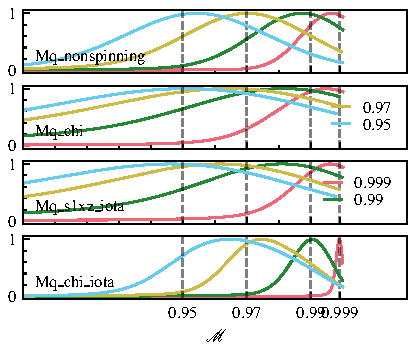
\includegraphics{metric_accuracy_hessian}
	\caption{Metric accuracy study for different manifolds.
	Each histogram shows the distribution of matches between $15000$ pairs of random points with metric match $0.95, 0.97, 0.99, 0.999$. The points are randomly drawn on the manifold with Eq.~\eqref{eq:tiling_pdf}.}
	\label{fig:metric_accuracy}
\end{figure}

\begin{figure}[t]
	\centering
	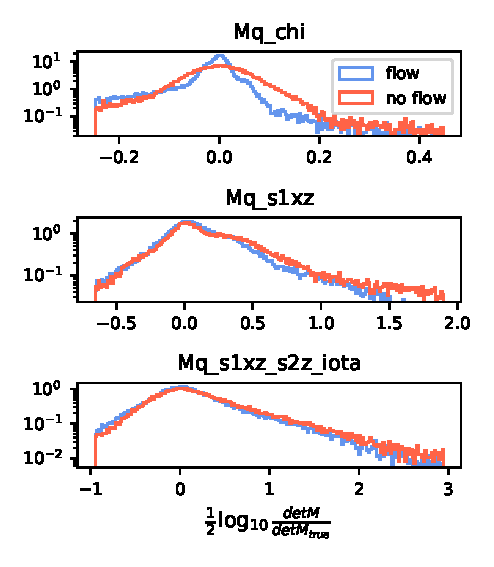
\includegraphics{tiling_validation}
	\caption{Histogram of the log ratio between the volume element approximated by the tiling $\sqrt{\text{det}M^\text{tiling}}$ and the un-approximated one. Each histogram is generated with $50000$ points. The tiling approximated metric does (label ``flow") and does not (label ``no flow") use the normalizing flow interpolation scheme.}
	\label{fig:tiling_validation}
\end{figure}

\begin{figure*}[th!]
	\centering
	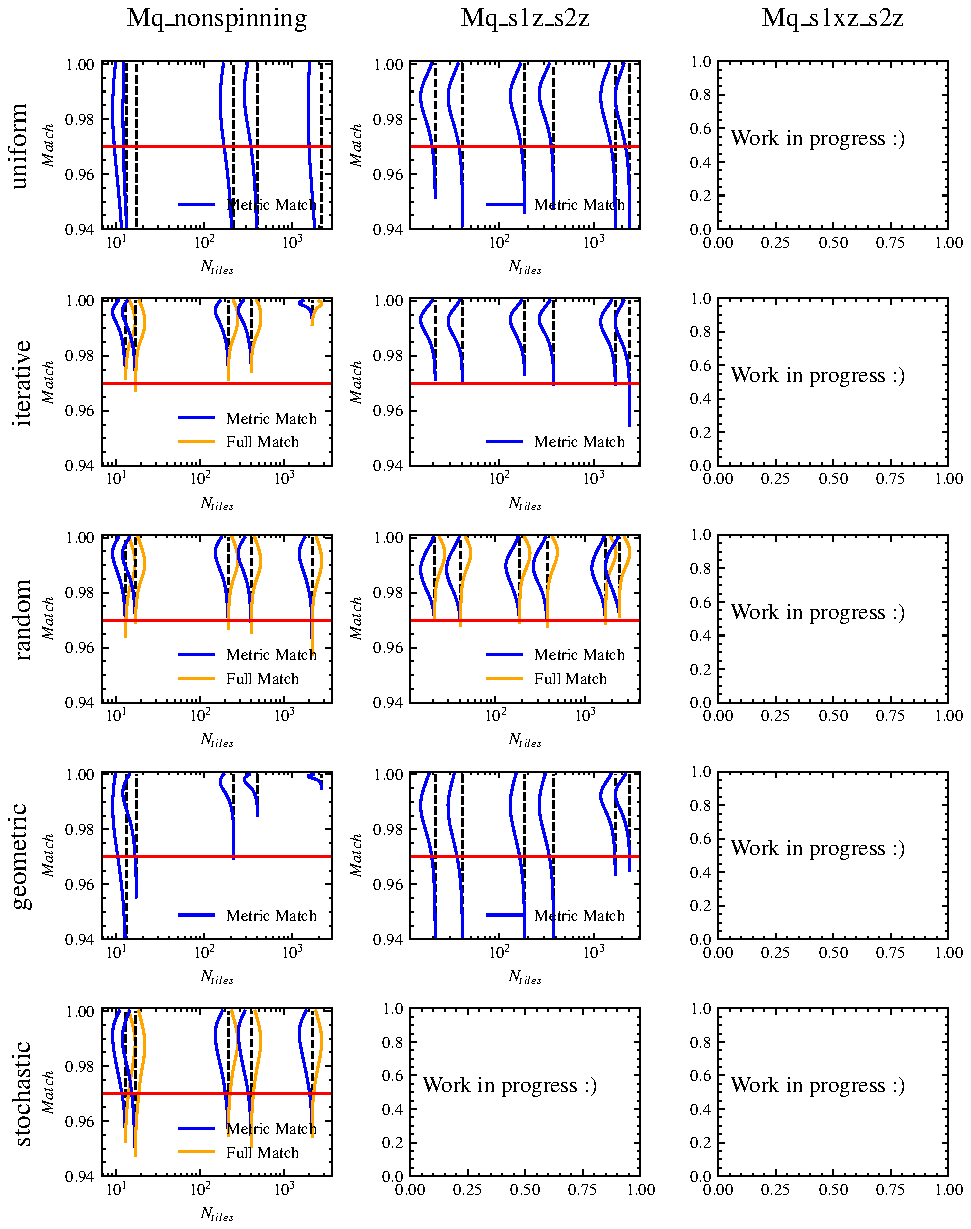
\includegraphics[width=.85\textwidth,keepaspectratio]{placing_validation}
	\caption{Results for the validation of the placing methods on $0.97$ minimum match banks. Each row refers to a different placing method whereas each column refers to a different manifold. In each plot, we report with a cross the number of tiles $N_{\text{tiles}}$ against the number of templates $N_{\text{templates}}$ of the bank.
	The diamond plot refers to the fitting factor distribution of an injection study performed on the banks. The fitting factor is computed both with the match (orange) and the metric match (blue). The histograms are normalized to arbitrary units and a red tick marks the $0.97$ match threshold. The upper limit of the histograms always corresponds to the match value of $1$ and the support extends until the 1st percentile of the distribution.
	The histograms are built with $1000$ injections for each bank.
	}
	\label{fig:placing_validation}
\end{figure*}

As the bank generation method relies on the assumption that the metric match provides a good approximation to the match, it is crucial to have a quantitative estimation of the goodness of this assumption.

To do this, we choose 4 different manifolds of templates $\mathcal{B}$ which cover different physical quantities of interests. For each manifold, we uniformly draw $15000$ samples on the manifold \textcolor{red}{uniformly draw them how? How have you distributed extrinsic parameters? It is common to do this uniform on the sky.}\textcolor{blue}{There are no extrinsic parameters involved here, as the injections are sampled from the manifold, which does not cover the sky location. Is that fine? I added a footnote above to clarify this point.} \textcolor{red}{If you compute the match with Eq. 5, do you not generate the waveforms? If you do, what is the complete set of waveform parameters?}and we compute the metric at each point.
For each point $\theta_C$, we pick a random point (again inside the manifold) at a constant metric match $\mathcal{M}_{\text{metric}}$ with respect to $\theta_C$\footnote{
This amounts to draw a point on the constant (metric) match ellipsoid centered in
$\theta_C$: $\{\theta \; | \; d_{\text{metric}}(\theta,\theta_C) \leq 1-\mathcal{M}_{\text{metric}} \}$.
}.
For each pair, we compute the match Eq.~\eqref{eq:match} and we plot the histogram of such values. For an increasingly accurate metric approximation, we should see an increasingly narrow histogram peaked around $M_{\text{metric}}$.
We repeat the experiment for $\mathcal{M}_{\text{metric}} = 0.95, 0.97, 0.99, 0.999$.

The experiment is performed on the following manifolds:
\begin{itemize}
	\item \texttt{Mq\_nonspinning} with coordinates $M = m_1+m_2, q = m_1/m_2>1$ in the rectangle $[20, 50] M_\odot \times [1,5]$ \textcolor{red}{maybe make these a bit more clear as to what variables these are. Also, are these all "rectangles"? Maybe should be hyperrectangles?}\textcolor{blue}{How about a "convention setup" section, to explain the meaning of all the variables? I did that in the text at beginning of section II but probably it can be highlighted more. I am using (this has just changed) all around the paper the term rectangle instead of hyperrectangle (the meaning seems obvious and it reads nicer). I'm happy to change this everywhere if you think it's the case.}
	\item \texttt{Mq\_chi} with coordinates $M, q, \chi = s_\text{1z} = s_\text{2z}$ in the rectangle $[20, 50] M_\odot \times [1,5] \times [-0.99, 0.99]$
	\item \texttt{Mq\_s1xz\_iota} with coordinates $M, q, s_\text{1}, \theta_1, \iota$ in the rectangle $[20, 50] M_\odot \times [1,5] \times [0, 0.99] \times [0,\pi]  \times [0,\pi]$, where $s_1, \theta_1$ are the polar coordinates of $(s_\text{1x}, s_\text{1z})$
	\item \texttt{Mq\_chi\_iota} with coordinates $M, q, \chi, \iota$ in the rectangle $[20, 50] M_\odot \times [1,5] \times [-0.99, 0.99] \times [0,\pi]$. We employ an higher-order-mode approximant
\end{itemize}

For the first two manifolds we use the approximant \texttt{IMRPhenomD} \cite{PhysRevD.93.044006, PhysRevD.93.044007}, whereas for the latter two we use \texttt{IMRPhenomPv2} \cite{PhysRevLett.113.151101} and \texttt{IMRPhenomXPHM} \cite{PhysRevD.103.104056} respectively. \textcolor{blue}{what stopping criteria and max-depth?}The frequency range for the metric computation is always $[10, 1024]Hz$.
The results are reported in Fig.~\ref{fig:metric_accuracy}.

%\begin{figure}[t]
%	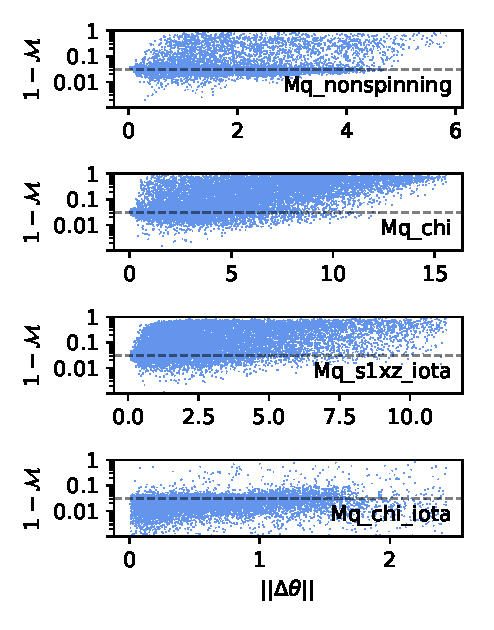
\includegraphics{metric_accuracy_hessian_distance}
%	\caption{For each pair of point with constant metric match of $0.97$ (i.e. mismatch of $0.03$, as marked by the dashed line), we report the actual mismatch as a function of coordinate distance $||\Delta\theta||$.
%	}
%	\label{fig:metric_accuracy_distance}
%\end{figure}
We first consider the first three manifolds covered with a non-HM approximant.
By looking at the results in Fig.~\ref{fig:metric_accuracy}, we note that all the histograms are very broad, showing a large discrepancy between the match and its metric approximation: the metric approximation does {\it not} provide a reliable estimation of the match. 
However, as will be shown in Sec.~\ref{sec:placing_accuracy}, such inaccuracy does not affect the quality of the generated template banks. Indeed, the primary quantity of interest for template placement is not the metric distance but the volume element $\sqrt{\text{det}M}$ of the manifold, which controls the template density. Clearly, the metric does not approximate well a single value for the distance but it is able to approximate the number of templates that should lay in a given volume, still providing reliable template banks.
In other words, the relative orientation of the eigenvectors of the metric (which determines the metric match) may be off but the magitude of the eigenvalues of the metric provides meaningful information, which is used by the template placing methods.
\stefano{Is this part better now?}
%
%However, as discussed above, the metric approximation  (Eq.~\eqref{eq:metric_definition}) to the match (Eq.~\eqref{eq:match}) comes from a Taylor expansion and it is guaranteed to be valid whenever the higher-order terms of the expansion are small (e.g. at third order $H^{(3)}_{ijk}\Delta\theta_i\Delta\theta_j\Delta\theta_k$). To quantify this, one should compute the full Taylor expansion, which is expensive and out of the scope of the work. We can limit ourselves to note that higher order terms tend to become negligible as $||\Delta\theta||$ becomes smaller.
%

The picture changes by inspecting the manifold \texttt{Mq\_chi\_iota}, which includes HMs.
The metric approximation consistently {\it underestimates} the match, providing a lower limit.
As we will see, this bias is consistent with the injection study for the HM bank generated in Sec.~\ref{sec:HM_bank}, which shows a large discrepancy between metric match and match.
The reason for such different qualitative behaviour, whenever HMs are included, is unknown and requires more investigation. 


\begin{table*}[t!]
	%\centering
	\setlength\extrarowheight{1pt}
	 \begin{tabular}{l l c c c c} 
	 \hline
	 	%header
	 \multicolumn{1}{c}{\phantom{Bank name}} & \multicolumn{1}{c}{\textbf{Ranges}} & 
	 \multicolumn{2}{c}{
		\begin{tabular}{c c} \multicolumn{2}{c}{\textbf{Size}}  \\ \texttt{sbank} & \texttt{mbank} \\ \end{tabular}	 
	 } &
	  \multicolumn{2}{c}{
		\begin{tabular}{c c} \multicolumn{2}{c}{\textbf{Time}}  \\ \texttt{sbank} & \texttt{mbank} \\ \end{tabular}	 
	 }\\	 
	 %\multicolumn{1}{c}{\phantom{Bank name}} & \multicolumn{1}{c}{\textbf{Ranges}} & \multicolumn{2}{c}{\textbf{Size}} \\	 
	 %\multicolumn{1}{c}{\phantom{Bank name}} & \multicolumn{1}{c}{\phantom{Ranges}} & \multicolumn{1}{c}{\texttt{sbank}} & \multicolumn{1}{c}{\texttt{mbank}} \\
	 \hline
	 Nonspinning & \begin{tabular}{@{}l@{}} $M\in [30,50] M_\odot$ \\ $q\in [1,5]$   \\ \end{tabular}  &
	 		396 & 371 & $O(\text{hours})$ & $O(\text{seconds})$ \\
	 \cdashline{1-6}
	 Aligned spin & \begin{tabular}{@{}l@{}} $M\in [30,50]$ \\ $q\in [1,5]$ \\ $s_\text{1z}, s_\text{2z}\in [-0.99,0.99]$  \\ \end{tabular}  &
	 	3275 & 4117 & $O(\text{days})$ & $O(\text{minutes})$ \\
	 \cdashline{1-6}
	 Aligned spin low mass & \begin{tabular}{@{}l@{}} $M\in [10,30]$ \\ $q\in [1,5]$ \\ $s_\text{1z}, s_\text{2z}\in [-0.99,0.99]$  \\ \end{tabular}  &
	 	62009 & 80524 & $O(\text{months})$ &  $O(\text{hours})$\\
	 \hline
	 \end{tabular}
	 \caption{Comparison between the performance of \texttt{mbank} and  \texttt{sbank} on 3 chosen template banks.
	 For each bank, we report the range of parameters covered by the templates, the size of the banks generated by the two methods, as well as the order of magnitude of the generation time. The frequency range for all the banks is $f\in [15,1024] Hz$.
	 The details of the injection studies are shown in figure~\ref{fig:sbank_comparison}.
	 The comparison are made on a machine with CPU Intel(R) Xeon(R) CPU E5-2630 installed.
	 }
 	 \label{tab:sbank_comparison}
\end{table*}

\subsection{Tiling accuracy} \label{sec:tiling_accuracy}

In this section, we evaluate the accuracy of the tiling approximation to the metric. To measure the discrepancy between the metric $M_{ij}$ Eq.~\eqref{eq:metric_expression} and its approximation $M^\text{tiling}_{ij}$, we look at the ratio between volume elements $0.5\log_{\textrm{10}}\frac{\text{det} M^\text{tiling}}{\text{det}M}$, similar to Eq.~\eqref{eq:stop_tiling}.
The metric approximated by the tiling is computed both with normalizing flow (Eq.~\eqref{eq:metric_flow}) and without normalizing flow (Eq.~\eqref{eq:metric_tiling}).

We consider three different manifolds:
\begin{itemize}
	\item \texttt{Mq\_chi} with coordinates $M, q, \chi $ in the rectangle $[40, 50] M_\odot \times [1,5] \times [-0.99, 0.99]$
	\item \texttt{Mq\_s1xz} with coordinates $M, q, s_{1}, \theta_1$ in the rectangle $[40, 50] M_\odot \times [1,5] \times [0, 0.99] \times [0,\pi]$
	\item \texttt{Mq\_s1xz\_s2z\_iota} with coordinates $M, q, s_{1}, \theta_1, s_\text{2z}, \iota$ in the rectangle $[40, 50] M_\odot \times [1,5] \times [0, 0.99] \times [0,\pi] \times [-0.99, 0.99] \times [0, \pi]$
\end{itemize}
For the first manifold we use the approximant \texttt{IMRPhenomD}, while we use \texttt{IMRPhenomPv2} for the others.
For each manifold, we generate a tiling with stopping criteria $\epsilon = 0.1$ and max-depth $= 10$.
To compute the metric, we use the PSD for Handford measured on the first three months of the third observing run (O3), as publicly released by the LVK collaboration \cite{O3a_PSDs}. We consider a frequency window of $[10, 1024]Hz$.
We then randomly draw $50000$ points from the tiling, at each point we compute the metric and its approximation given by the tiling (with and without normalizing flow) and we finally compute the ratio between volume elements.

We present our results in Fig.~\ref{fig:tiling_validation}.
First of all, we note that all the histograms peak around $0$, as expected: this means that for the majority of points in the manifold, the tiling is able to provide an accurate approximation (within a order of magnitude) to the volume element.
Second, we see that all the histograms are not symmetric around their peak at $0$: the tiling approximation to the metric is more likely to {\it overestimate} the value of the volume element. When it comes to template placing, this translates into being more likely to have {\it over-dense} regions, which does not affect the recovery of the template bank but only its size.
Finally, the normalizing flow interpolation provides slightly more accurate results, yielding shorter tails in the ratio of volume elements: it is then useful to leverage the normalizing flow interpolation to achieve better performance.


\subsection{Placing methods accuracy} \label{sec:placing_accuracy}

Here we compare the properties of different placing methods: \textit{uniform}, \textit{random} and \textit{stochastic}.
This will be helpful to understand their ranges of applicability and possible limitations in their use.

We consider the three manifolds described above: \texttt{Mq\_chi}, \texttt{Mq\_s1xz} and \texttt{Mq\_s1xz\_s2z\_iota}.
For each manifold, we generate several tilings with a different number of tiles (obtained setting a different value of max-depth) and we generate a bank with $0.97$ minimum match.
We will {\it not} use a normalizing flow model to interpolate the metric.

We report the histogram of the fitting factors for both the match and the metric match, computed on a set of $1000$ injections.
We stop the stochastic placement algorithm after $N_\text{max} = 200$ iterations with no new templates, while for the random method we employ $10000$ livepoints.
The results are shown in Fig.~\ref{fig:placing_validation}.

According to Eq.~\eqref{eq:N_templates}, the number of templates $N_{\text{templates}}$ placed by the {\it uniform} method is a measure of the volume of the space. For this reason, it is interesting to look how the number of templates placed by the {\it uniform} method depends on the number of tiles.
We note that $N_{\text{templates}}$ grows with the number of tiles until a certain upper limit. This behaviour is expected, as an increasing number of tiles provides a better estimation of the overall volume of the space, until the estimation converges to the true value in the limit of many tiles. 

Depending on the dimensionality of the manifold, the different placing methods have different performance.
In the low dimensional manifolds \texttt{Mq\_chi} ($D=3$) and \texttt{Mq\_s1xz} ($D=4$), the {\it uniform} method has very poor performance and underestimates the number of templates. In the same two manifolds, the {\it stochastic} method performs very well and the {\it random} method gives a satisfying injection recovery, at the price of a large number of templates (3 times larger than those placed by the stochastic method).

The situation changes for the manifold \texttt{Mq\_s1xz\_s2z\_iota} ($D=6$), where the three methods show similar properties. The best performance is achieved by the {\it random} method, once again, at the cost of a large number of templates.
This is obtained thanks to the iterative control of the bank coverage, made by means of livepoints. On the other hand, since there is no control of the mutual distance between a proposal and the rest of the bank, it is very likely that some regions will be overcovered (i.e. some templates will be too close to each other).
Unlike the other examples, the {\it uniform} method shows similar features as the {\it stochastic} method, both in terms of template number and injection recovery.

The key observation is that in high dimensions, the control over the spacing of the templates performed by the {\it stochastic} method is not crucial anymore and provides only moderate improvement (or no improvement at all) over {\it uniform} or {\it random} methods. As discussed before, this is a well-known feature \cite{Messenger:2008ta, Allen:2021yuy, Allen:2022lqr} of high dimensional template banks and it makes the {\it random} (and similarly the {\it uniform}) method very appealing to cover a high dimensional region of the parameter space.

As a final remark, we note that the fitting factors computed with the metric match are widely consistent with the un-approximated ones. This shows the robustness of the metric approximation, despite the problems highlighted in Sec.~\ref{sec:metric_accuracy}. \textcolor{red}{okay, this is a very nice result; I want to understand better how this is possible despite the problems.} \stefano{We discussed it with Bhooshan, we can dive more into that}

%An analysis of the different methods shows that the {\it uniform} placing method has a poor performance for the low dimensional manifolds \texttt{Mq\_chi} and \texttt{Mq\_s1xz}, while still provides acceptable injection recovery for the large dimensional manifold \texttt{Mq\_s1xz\_s2z\_iota}. This was widely expcted. In low dimenensional manifolds, Eq.~\eqref{eq:N_templates} undestimates the number of templates and, since it does not check for boundaries, it provides poor coverage. This changes for high dimensional manifold, where the number of templates placed is consistent with the other methods and the coverage is satisfying, As discussed before, this is a well known features \cite{Messenger:2008ta, Allen:2021yuy, Allen:2022lqr} of high dimensional template banks and it makes the unform (and similarly the random) method very appealing to cover quickly a high dimensional region of the parameter space.

%The {\it random} method provides a very high injection recovery at the price of a very large number of templates. As shown in Fig.~\ref{fig:placing_validation}, manifolds \texttt{Mq\_s1xz} and \texttt{Mq\_s1xz\_s2z\_iota} are covered with around three times more templates than those placed by the other methods.The improved over the {\it uniform} method are obtained thanks to the iterative control of the bank coverage, made by means of livepoints. On the other hand, since there is no control of the mutual distance between a proposal and the rest of the bank, it is very likely that some regions will be overcovered (i.e. some templates will be too close to each other).

%The {\it stochastic} method is able to cover the low dimensional manifold with the appropriate minimum match. Moreover, the bank size does not depend on the number of tiles. This very nice performance is expected: this placing method (with some variations) is the state of the art of bank generation and has proven to be reliable in past years. The price to pay for such nice performance is a larger bank generation time when compared with the other two methods: indeed, a lot of computational power is spent on computing mutual distances between the templates, which makes this method slower and at the same time more accurate.


\begin{figure}[t!]
	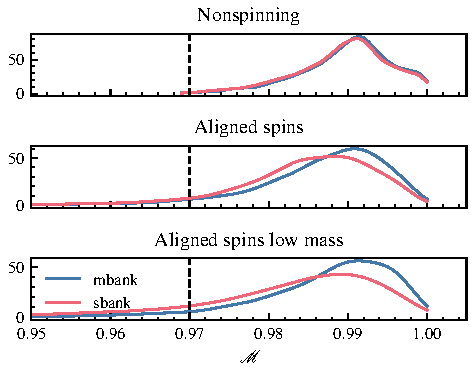
\includegraphics{sbank_comparison}
	\caption{
	Cumulative distribution of the fitting factors of the banks used to compare \texttt{mbank} and \texttt{sbank}. For each parameter space considered, we randomly draw $5000$ points (injections) from the tiling used to generate the \texttt{mbank} bank and we compute the fitting factor of these injections against the two banks. We report the distribution of fitting factor in the histograms. For visualization purposes, we plot the $0.97$ line, which corresponds to the minimum match of the banks.
	The details of the banks generated are reported in Tab.~\ref{tab:sbank_comparison}.
	}
	\label{fig:sbank_comparison}
\end{figure}

\begin{figure}[t!]
	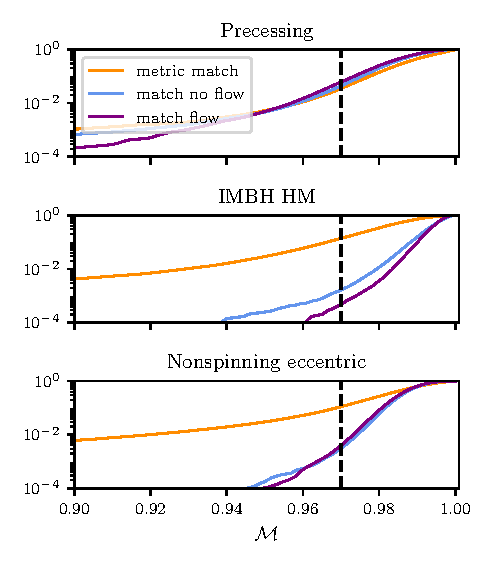
\includegraphics{bank_injections_flow}
	\caption{
	Cumulative distribution of the fitting factors of the three case study banks. Each bank is generated with the normalizing flow interpolation (label ``flow") and without (label ``no flow"). For each bank, we randomly draw $75000$ points (injections) from the tiling and we compute the fitting factor of these injections against the two banks. We report the distribution of fitting factor in the histograms both for the match (both cases) and the metric match (only ``no flow" case). For visualization purposes, we plot the $0.97$ line, which corresponds to the minimum match of the banks.
	The details of the banks generated are reported in Tab.~\ref{tab:casestudy_banks}.
	%\stefano{Should we make the histogram of the cumulative distribution of the match values? Maybe it's more informative}
	}
	\label{fig:bank_injections}
\end{figure}

\subsection{Comparison with \texttt{sbank} }\label{sec:sbank_comparison}

The stochastic template placement code \texttt{sbank} \cite{Ajith:2012mn} is a very common tool used by the LIGO Scientific, Virgo and Kagra Collaborations (LVK) to generate large template banks for analysis and, as such, it has been successfully used in the past three observing runs by several search pipelines for compact binary coalescence \cite{Usman:2015kfa, Mukherjee:2018yra, Aubin:2020goo} \textcolor{blue}{More references?}.
For this reason, it is very important to compare the performance of our code against \texttt{sbank}. The comparison is based on the size, speed and effectualness of the banks generated.

We generate three non-precessing template banks with both \texttt{sbank} and \texttt{mbank}:
\begin{itemize}
	\item A {\it non-spinning} bank
	\item An {\it aligned-spin high-mass} bank
	\item An {\it aligned-spin low-mass} bank
\end{itemize}
The ranges of the parameter space covered by the three banks are reported in Tab.~\ref{tab:sbank_comparison}. All the banks cover the frequency range $f\in [15,1024] Hz$ and are generated using the PSD measured during the whole second observing run (O2).
For all the three banks, \texttt{mbank} templates are placed with the {\it stochastic} method, with $N_\text{max}=300$ and without the use of a normalizing flow model to interpolate the metric. In Fig.~\ref{fig:sbank_comparison}, we report the result of an injection study on the three pairs of banks.

By looking at the banks' size in Tab.~\ref{tab:sbank_comparison}, we observe that \texttt{mbank} consistently places around 30\% more templates than \texttt{sbank}, in the two aligned spins banks. This means that the metric template placement tends to \textit{overcover} the space: it is a known feature (also observed in \cite{Coogan:2022qxs}) and it is inherent to the use of a metric approximation: it is the price to pay for a huge speed-up in the generation.

Looking at the injections fitting factor distributions in Fig.~\ref{fig:sbank_comparison}, we note the fitting factor distribution of \texttt{sbank} and \texttt{mbank} are similar in their shape, even though \texttt{sbank} shows a slightly better performance than \texttt{mbank} in two cases. This suggests that, at least in this simple non-precessing parameter space, \texttt{mbank} is able to match the state-of-the-art performance in covering, in a fraction of the computing time.

%When considering the generation times, we see that \texttt{mbank} is {\it orders of magnitude} faster than \texttt{sbank}. This huge speed up is precisely what makes \texttt{mbank} convenient, especially to cover very large volumes: it may overcover the space but it provides a substantial speed-up, making feasible the covering of new regions of the parameter space.

%%%%%%%%%%%%%%%%%%%%%%%%%%%%%%%%%%%%%%%%%%%%%%%%%%%%%%%


\begin{table*}[t!]
	\centering
	\setlength\extrarowheight{1pt}
	 \begin{tabular}{l l l c c c} 
	 \hline
	 %\multicolumn{1}{c}{\phantom{Name}} & \multicolumn{1}{c}{\textbf{Ranges}} & \multicolumn{1}{c}{\textbf{Setting}} & \multicolumn{1}{c}{\textbf{Size}} \\
	 \multicolumn{1}{c}{\phantom{Bank name}} & \multicolumn{1}{c}{\textbf{Ranges}} & \multicolumn{1}{c}{\textbf{Settings}} &  
	 \multicolumn{2}{c}{
		\begin{tabular}{c c} \multicolumn{2}{c}{\textbf{Size}}  \\ $N_{\text{tiles}}$ & $N_{\text{templates}}$ \\ \end{tabular}	 
	 } &
	 \multicolumn{1}{c}{
		\begin{tabular}{c} \multicolumn{1}{c}{\textbf{Size (flow)}}  \\ $N_{\text{templates}}$ \\ \end{tabular}	 
	 } \\
	 \hline
	 Precessing & \begin{tabular}{@{}l@{}} $M\in [25,100] M_\odot$ \\ $q\in [1,5]$  \\ $s_1\in [0,0.99]$ \\$\theta_1\in [0, \pi]$ \\ $f\in [15,1024] Hz$ \end{tabular}  &
	 \begin{tabular}{@{}l@{}} IMRPhenomPv2 \\ $\epsilon = 0.1$ \\ max-depth: 10 \\ $N_\text{max} = 200$ \\ $n_\text{layers} = 6$ \\ $n_\text{hidden} = 6$ \end{tabular}  &
	 33774 & 54923 & 51953\\
	 \cdashline{1-6}
	 IMBH HM & \begin{tabular}{@{}l@{}} $M\in [50, 600] M_\odot$ \\ $q\in [1,5]$  \\ $\chi \in [0,0.99]$ \\ $f\in [10,1024] Hz$ \\ \end{tabular}  &
	 	 \begin{tabular}{@{}l@{}} IMRPhenomXPHM \\ $\epsilon = 0.2 $ \\ max-depth: 8 \\ $N_\text{max} = 100$\\ $n_\text{layers} = 6$ \\ $n_\text{hidden} = 6$ \end{tabular}  &
	 	33792 & 168010 & 134326\\
	 \cdashline{1-6}
	 Nonspinning eccentric & \begin{tabular}{@{}l@{}} $M\in [10,75] M_\odot$ \\ $q\in [1,5]$ \\ $e \in [0,0.3]$ \\ $f\in [15,1024] Hz$ \\ \end{tabular}  &
	 	 \begin{tabular}{@{}l@{}} EccentricFD \\ $\epsilon = 0.1$ \\ max-depth: 9 \\ $N_\text{max} = 100$\\ $n_\text{layers} = 2$ \\ $n_\text{hidden} = 4$ \end{tabular}  &
	 	4238 & 115748 & 104210\\
	 \hline
	 \end{tabular}
	 \caption{Summary of three case study banks generate with \texttt{mbank}. For each bank generated, we report the variables being sampled and their ranges. We also report the approximant and the hyperparameters $\epsilon$ and max-depth used for the tiling generation as well as the bank size $N_{\text{templates}}$, the number of tiles $N_{\text{tiles}}$ and the architecture of the normalizing flow used. Results of an injection study are shown in Fig.~\ref{fig:bank_injections}. The templates distribution of the three banks is reported in Fig.~\ref{fig:bank_scatter}.}
 	 \label{tab:casestudy_banks}
\end{table*}


\begin{figure*}[t]
	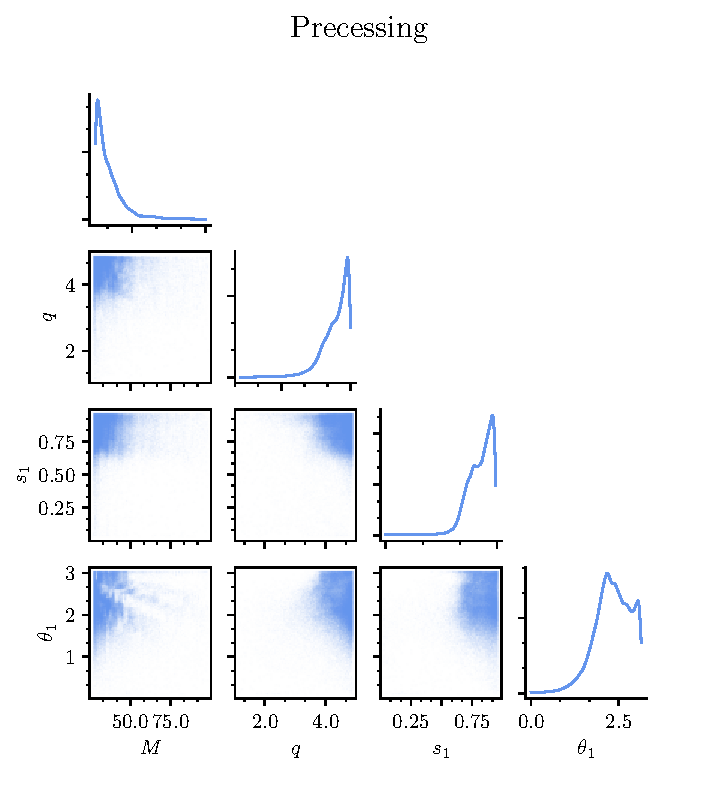
\includegraphics[scale = 0.7]{bank_scatter_Precessing}\hfill
	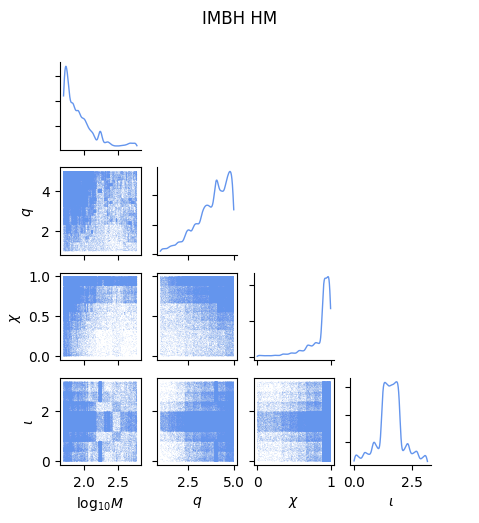
\includegraphics[scale = 0.7]{bank_scatter_IMBH_HM}\hfill
	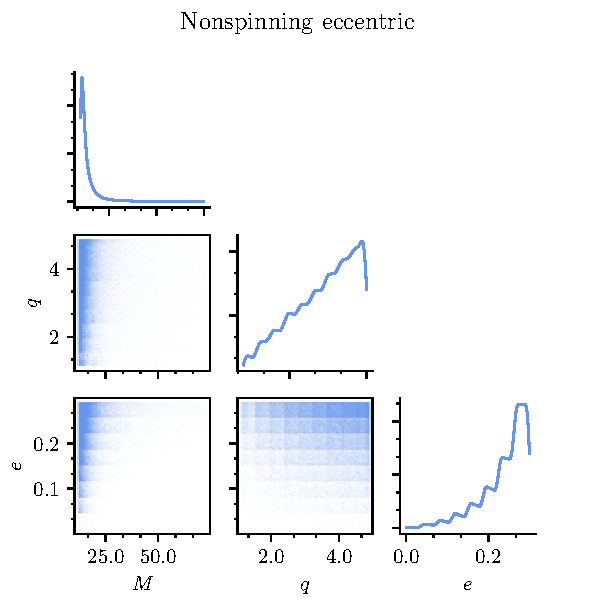
\includegraphics[scale = 0.7]{bank_scatter_Nonspinning_eccentric}
	\caption{Corner plots showing the templates for the three banks described in Tab.~\ref{tab:casestudy_banks}, {\it without} using normalizing flow interpolation. The masses of each template are parametrized with total mass $M$ and mass ratio $q>1$. In the precessing bank, the spin of the first BH is described by its magnitude $s_1$ and the in-plane angle $\theta_1$. In the HM bank, the templates are described by the effective spin parameter $\chi = s_\text{1z} = s_\text{2z}$ and by the inclination angle $\iota$. In the eccentric bank, besides the masses, we only consider the eccentricity $e$ of the system.}
	\label{fig:bank_scatter}
\end{figure*}

\begin{figure*}[t]
	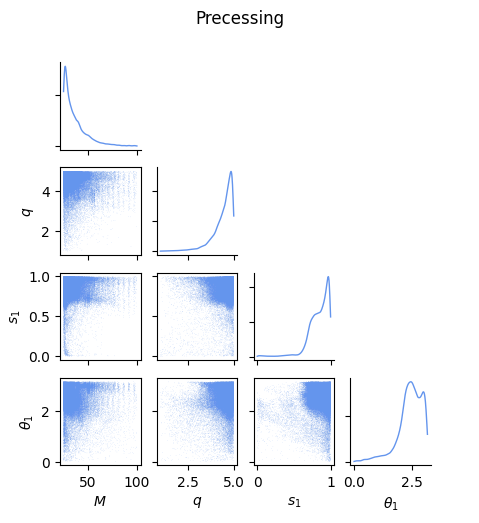
\includegraphics[scale = 0.7]{bank_scatter_Precessing_flow}\hfill
	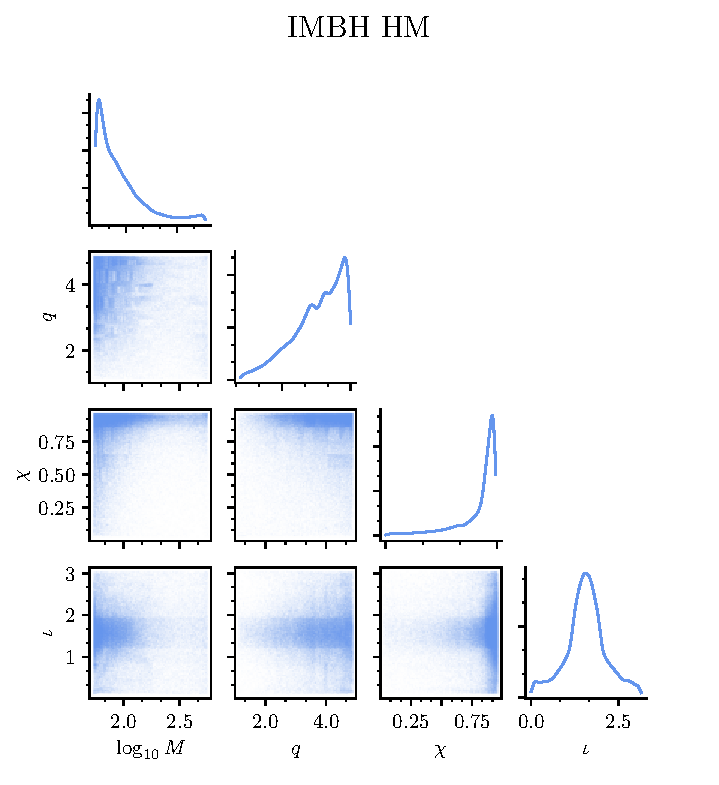
\includegraphics[scale = 0.7]{bank_scatter_IMBH_HM_flow}\hfill
	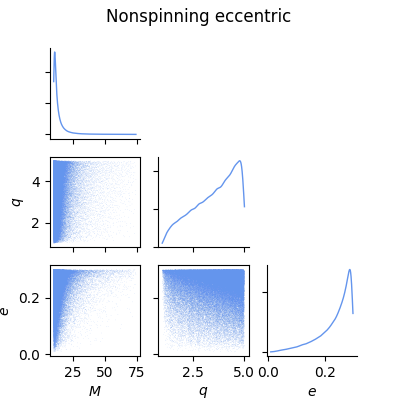
\includegraphics[scale = 0.7]{bank_scatter_Nonspinning_eccentric_flow}
	\caption{Corner plots showing the templates for the three banks described in Tab.~\ref{tab:casestudy_banks}, using normalizing flow interpolation. The templates are parametrized in the same way of Fig.~\ref{fig:bank_scatter}.}
	\label{fig:bank_scatter_flow}
\end{figure*}

	%%%%%%%%%%%%%%%%%%%%%%%%%%%%%%%%%
\section{Bank generation: three case studies} \label{sec:bank_generation}

To demonstrate the capabilities of our method, we use \texttt{mbank} to generate three large banks, covering interesting regions of the parameter space:
	\begin{itemize}
		\item A precessing BBH bank
		\item An IMBH bank with HMs
		\item A nonspinning BBH eccentric bank
	\end{itemize}
We generate two versions of each bank, one with normalizing flow interpolation of the metric (``flow" bank) and one without (``no flow" bank).
%Generating these banks with a standard approach is extremely costly and they represent the ideal situation where \texttt{mbank} is useful.

For each bank, we perform an injection study with $75000$ injections: the results are reported in Fig.~\ref{fig:bank_injections}. We also plot the templates of the banks in Fig.~\ref{fig:bank_scatter} (without normalizing flow interpolation) and in Fig.~\ref{fig:bank_scatter_flow} (with normalizing flow interpolation).
In Tab.~\ref{tab:casestudy_banks}, we summarize the features of each bank, such as the size and the range of physical quantities that they cover.
All the banks are generated with a minimum match $MM$ requirement of $0.97$, using the {\it stochastic} placement method.
As above, we use the Hanford detector PSD measured during O3, as publicly released by the LVK collaboration \cite{O3a_PSDs}.

\subsection{A precessing bank}\label{sec:precessing_bank}
	
In our high mass {\it precessing} bank, we assign a two dimensional precessing spin to the most massive BH, by considering only the x and z components of the spin $s_1$, sampled in polar coordinates. The masses are sampled in the space (total mass - mass ratio) $M,q$.  Thus the metric is evaluated at the coordinates point $\theta = (M, q, s_1, \theta_1)$. We use the approximant \texttt{IMRPhenomPv2}.

This choice of variable is based on the fact that the effect of precession can be absorbed in a single {\it effective spin parameter}, assigned to the most massive BH of a binary \cite{PhysRevD.91.024043, PhysRevD.103.083022}. Hence this physical approximation allows us to cover a large number or precessing signal using a (relatively) small number of variables.

By looking at the scatter plots of the templates Fig.~\ref{fig:bank_scatter}, it is manifest the effect due to the discretization error introduced by the tiles: this causes a discontinuity in the template density. Of course, this effect is unphysical and would have been avoided by a purely stochastic placing method.
Another possible source of discontinuity can be traced back to numerical noise in the numerical gradients of the waveforms. Depending on the approximant, the gradients (hence the metric) may not behave smoothly all across the parameter space, thus explaining (partly) the hard discontinuities.

The normalizing flow interpolation removes the discontinuities in the template densities. Moreover, it generates a bank with a smaller number of templates, arguably due to a reduction of overcoverage around the boundaries of each tile. This feature is consistent across all the other two banks generated.

The injection recovery (Fig.~\ref{fig:bank_injections}) is satisfying for both the precessing banks, with less than $10\%$ of the $75000$ injections performed having a recovery less than the target match $MM = 0.97$ (for the ``no flow" case). The ``flow" case show a consistent histogram.
We also note that the fitting approximated by the metric are consistent between with the un-approximates ones.
The bank coverage can be straightforwardly improved by setting a more stringent termination requirement $N_\text{max}$, which will add more templates with an improvement in injection recovery.

\subsection{An IMBH HM bank}\label{sec:HM_bank}

We generate a bank, covering part of the IMBH region, that includes Higher Order Modes. As HMs are more important in the strong gravity regime, they affect mostly the late inspiral and the merger part of the waveform.
For this reason, it is interesting to search HM data in the IMBH region, characterized by a total mass $M>50 M_\odot$. An IMBH signal spends only a small time ($O(ms)$) in the detector's frequency band and thus an accurate HM template is crucial for better detection.
We include in the bank the variables $\log M, q, \chi, \iota$, where $\chi=s_\text{1z}=s_\text{s2z}$ is the effective spin parameter and $\iota$ is the inclination angle.
As before in Tab.~\ref{tab:sbank_comparison}, we report the ranges for each of this quantities. We use the modern HM approximant \texttt{IMRPhenomXPHM}.

The inclusion of HM makes the bank much larger (in other words the volume of the space is larger): for reference, a non HM bank, covering the masses and $\chi$ ranges (of course, without $\iota$) has $\sim 1000$ templates: that is a 2 orders of magnitude difference!

By looking at the injection recovery Fig.~\ref{fig:bank_injections} it is striking the discrepancy between the fitting factor computed by the metric and the un-approximated one. Indeed, in the HM case the metric strongly {\it underestimates} the match, yielding an overpopulated bank. For the ``no flow" case, approximately $12\%$ of the injections have a {\it metric} match recovery below $0.97$: this is consistent with the placing method used, which only ``knows" about metric matches. On the other hand, only $\sim 0.3\%$ are below the $0.98$ recovery factor: the bank generated is effectively a $98\%$ bank.
This effect is consistent with what observed in Fig.~\ref{fig:metric_accuracy} and it is only observed whenever an HM approximant is used: as discussed above, the cause of this is unknown and requires more investigation.

As above, the ``flow" case has less templates with a similar injection recovery and removes the discontinuities in template density.

\subsection{An eccentric nonspinning bank}\label{sec:eccentric_bank}

Usually the BBH searches have focused on circular orbits.
This is well theoretically motivated, as by the time of merger, any initial orbital eccentricty will be radiated away. Nevertheless is interesting to search such signals as their detection will provide invaluable information on the BBH dynamics and the BBH formation channels and stellar evolution.
The eccentricity leaves a characteristic signature on the inspiral, thus it will be more detectable on long signals. For this reason, we focus on the {\it low} mass region $M\in [10,75] M_\odot$, where the inspiral is detectable for a longer time.
To generate our eccentric bank, we use the approximant \texttt{EccentricFD} \cite{PhysRevD.93.124061} and we limit ourself to low eccentricities $e<0.3$, where the WF modelling is more reliable. Being a Post-Newtonian model, it does not include the merger and the waveform are cut in the late inspiral, as done by the code \texttt{lalsimulation} \cite{lalsuite}. Of course, this removes interesting physics and the resulting bank is expected to have a lower number of templates than what obtained using a fully eccentric approximant.

As in the case of the HM bank, the addition of eccentricity delivers a bank orders of magnitude larger than a standard non-eccentric bank.
Moreover, by looking at the fitting factor distributions, we note that, similarly to the IMBH case, the metric {\it underestimates} the match. Again, the origin of this is still under investigation.

From the scatter plot Fig.~\ref{fig:bank_scatter}, we note that the discontinuities introduced by the metric are less visible. This is due to the smaller dimension of the space (3 against 4 of the previous cases), which makes easier to cover the space with a reliable tiling. Moreover, since the approximant \texttt{EccentricFD} is analytic, the metric has a smoother dependence on the parameter space, which may also help to avoid discontinuities in template density.
As in all other cases, the normalizing flow interpolation effectively removes this feature.

\section{Final remarks and future prospects} \label{sec:conclusion}

We present a novel method to generate template banks to cover a high dimensional manifold of (possibly) precessing/HM/eccentric BBH signals.
We rely on the metric approximation to the match Eq.~\eqref{eq:metric_definition} to compute distances between points and we set up an algorithm to create a tiling of the manifold. Given a tiling, we are able to implement several strategies to place templates to cover the space with a given minimum match target.
A normalizing flow model can be optionally used to interpolate the metric, providing a more efficient coverage.
The code implementing our method is publicly available as a package \texttt{mbank} and it comes with a number of tools to make the bank generation and validation easy.

To validate our method, we compare the output of our code to the one of the state-of-the-art \texttt{sbank}: we find that mbank is able to faithfully cover the space, although with a larger number of templates when compared with \texttt{sbank}.
To demonstrate the capabilities of our code, we generated three banks covering some interesting and up to now unexplored regions of the parameter space. We found the \texttt{mbank} is able to provide a faithfully coverage.
The banks generated are ready to be employed in real GW searches.

\texttt{mbank} is order of magnitude faster than the non-metric state-of-the-art bank generation codes. This makes our code particularly suitable for a large dimensional parameter space and makes feasible the generation of banks for which the template placing was hitherto unfeasible, due to computational limitations.
This was possible thanks to three innovative features:
\begin{itemize}
	\item The metric is used consistently everywhere throughout the package
	\item The tiling provides a fast and efficient interface to the metric, making tractable hard problems such as volume estimation and manifold sampling.
	\item The normalizing flow model is able to faithfully reproduce the volume element around the parameter space
\end{itemize}

Our work can be improved and extended in several directions:
\begin{itemize}
	\item {\it Improving the metric computation}. As discussed in Sec.~\ref{sec:metric_accuracy}, the metric accuracy may not be optimal, especially for large coordinate distance $||\Delta\theta||$. While this has proven not to affect negatively the template placing, it would still be desiderable to have a better estimation of the match. Future developments can work in this direction by solving the problem in Eq.~\eqref{eq:metric_optmization} or even departing from the bilinear approximation\footnote{
Although this latter strategy may sound tempting, it would cease to provide a meaningful estimation of volume, which may be problematic for template placement.} of Eq.~\eqref{eq:metric_definition}.
	
	\item {\it Investigate the performance for HM}. We observed in Sec.~\ref{sec:HM_bank} that the metric placement overcovers the space, due to the fact that the metric underestimates the match. This is puzzling and it requires more investigation.
	
	\item {\it Post process the bank}. Regardless of the placing method, the templates in a bank may not be placed optimally, creating over(under)dense regions. This is especially true for the {\it random} placing method. It may be good to add a post-processing step to move or remove some templates. The overall result can be a smaller bank with better covering properties \cite{Indik:2017vqq}.
\end{itemize}

As a final remark, we emphasize that our work enables the GW community to run searches on novel regions of the BBH signals parameter space. By cutting the bank generation and validation time by orders of magnitude, the computational cost of searching new regions of the parameter space will be dominated by the actual cost of the analysis rather than the cost of prior steps.
This will allow for optimal resource allocation to search for signature of precession, eccentricity and/or HMs, hopefully leading to new exciting physics discovery.

	%%%%%%%%%%%%%%%%%%%%%%%%%%%%%%%%% ACKNOWLEDGMENTS
        \begin{acknowledgments}
		S.S. and S.C. are supported by the research program of the Netherlands Organisation for Scientific Research (NWO).
		The authors are grateful for computational resources provided by the LIGO Laboratory and supported by the National Science Foundation Grants No. PHY-0757058 and No. PHY-0823459. This material is based upon work supported by NSF’s LIGO Laboratory which is a major facility fully funded by the National Science Foundation.
%		We thank Melissa Lopez Portilla, Aaron Zimmerman and Keith Riles for precious comments.
        \end{acknowledgments}

	%%%%%%%%%%%%%%%%%%%%%%%%%%%%%%%%% APPENDIX
%\newpage
\appendix
\section{Details of the metric computation}\label{app:metric}

In this appendix we report the details of the derivation of the Eq.~\eqref{eq:metric_expression}, as well as the computation of the Hessian $H$ of the overlap Eq.~\eqref{eq:overlap} in terms of the gradients of the waveform $h(\theta)$. 
In what follows, we define $\rescalar{h_1}{h_2}$ and $\imscalar{h_1}{h_2}$ to be respectively the real and imaginary part of $\scalar{h_1}{h_2}$.

We begin by expanding the quantity $\mathcal{M}(\theta,\theta +\Delta\theta)$ for $\Delta\theta$ around $0$. Since the $\mathcal{M}(\theta,\theta +\Delta\theta)$ has a maximum for $\Delta\theta = 0$, the leading term is quadratic in $\Delta\theta$.
We obtain:
\begin{align} \label{eq:metric_derivation}
	&\mathcal{M}(\theta,\theta +\Delta\theta) = \max_{\Delta t} \mathcal{O}(\theta, \theta + \Delta\theta, \Delta t) \nonumber\\
	& =	\max_{\Delta t} \left\{ 1+ \frac{1}{2}\left[ \partial_{ij}\mathcal{O} \Delta\theta_i \Delta\theta_j + 2  \partial_{it}\mathcal{O} \Delta\theta_i \Delta t + \partial_{tt}\mathcal{O} (\Delta t)^2 \right] \right\}  \nonumber \\
	&= 1 + \frac{1}{2}\left[ \partial_{ij}\mathcal{O} - \frac{\partial_{it}\mathcal{O} \partial_{jt}\mathcal{O}}{\partial_{tt}\mathcal{O}}\right] \Delta\theta_i \Delta\theta_j
\end{align}
where all the derivatives are evaluated at ${\Delta\theta = \Delta t = 0}$ and the explicit time maximization yields
${\Delta t = -\frac{\partial_{it}\mathcal{O} \Delta\theta_i}{\partial_{tt}\mathcal{O}}}$.

From the above Eq.~\eqref{eq:metric_derivation}, we can read the expression for the metric in Eq.~\eqref{eq:metric_expression} recognizing in the derivatives $\partial\partial\mathcal{O}|_{\Delta\theta, \Delta t = 0}$ the components of the Hessian matrix $H$ of the overlap.

We now compute the Hessian of the overlap as a function of the gradients of the {\it normalized} waveforms.
We have\footnote{
A constant factor in front of the frequency in the fourier transform does not affect the result. For this reason, we dropped the constant $2\pi$ in the exponential.}:
\begin{align}
	\partial_i \mathcal{O} &= \frac{1}{\mathcal{O}} \left[ \rescalar{\hat{h}}{\hat{h}e^{ift}}\rescalar{\hat{h}}{\partial_i\hat{h}e^{ift}} + \imscalar{\hat{h}}{\hat{h}e^{ift}}\imscalar{\hat{h}}{\partial_i\hat{h}e^{ift}} \right]\\
	\partial_t \mathcal{O} &= \frac{1}{\mathcal{O}} \left[ \rescalar{\hat{h}}{\hat{h}e^{ift}}\rescalar{\hat{h}}{\hat{h}if e^{ift}} + \imscalar{\hat{h}}{\hat{h}e^{ift}}\imscalar{\hat{h}}{\hat{h}if e^{ift}} \right]
\end{align}
Differentiating another time, after some rearrangements, we get:
\begin{align}
H_{tt} &= \frac{\partial^2 \mathcal{O}}{\partial t \partial t } \left|_{\Delta\theta, t = 0} \right.
								= \rescalar{\hat{h}}{\hat{h}f}^2 - \rescalar{\hat{h}}{\hat{h}f^2} \label{eq:H_tt}\\
H_{ti} &= \frac{\partial^2 \mathcal{O}}{\partial \Delta \theta_i \partial t } \left|_{\Delta\theta, t = 0} \right.
								= - \imscalar{\hat{h}}{\partial_i \hat{h}f} + \imscalar{\hat{h}}{\partial_i\hat{h}} \rescalar{\hat{h}}{\hat{h}f} \label{eq:H_ti}\\
H_{ij} &= \frac{\partial^2 \mathcal{O}}{\partial \Delta \theta_i \partial \Delta \theta_j }\left|_{\Delta\theta, t = 0} \right.
								= \rescalar{\hat{h}}{\partial_i\partial_j\hat{h}} +\imscalar{\hat{h}}{\partial_i\hat{h}} \imscalar{\hat{h}}{\partial_j\hat{h}} \label{eq:H_ij}
\end{align}

To move further, we express the normalized waveform derivatives in terms of the non normalized ones:
\begin{align*}
	\bullet&\quad \partial_i \scalar{h}{h} = \scalar{\partial_i h}{h}+ \scalar{h}{\partial_i h} = 2 \rescalar{h}{\partial_i h} \\
	\bullet&\quad \partial_i \hat{h} =\frac{1}{\rescalar{h}{h}^{3/2}} \left[ \rescalar{h}{h}\partial_i h -  \rescalar{h}{\partial_i h} h \right]	\\
	\bullet &\quad \partial_i \partial_j \hat{h} = \frac{1}{\rescalar{h}{h}^{1/2}} \partial_{ij}h 	+3 \frac{1}{\rescalar{h}{h}^{5/2}} \rescalar{h}{\partial_i h}\rescalar{h}{\partial_j h}h \\
	&- \frac{1}{\rescalar{h}{h}^{3/2}} \left[\rescalar{h}{ \partial_{ij} h} h + \rescalar{\partial_i h}{\partial_j h}  h
		+2\rescalar{h}{\partial_{(i} h} \partial_{j)} h \right]
\end{align*}
where $A_{(ij)} = \frac{1}{2}(A_{ij}+A_{ji})$ denotes symmetrization.

Plugging this into the equations~\eqref{eq:H_tt}-\eqref{eq:H_ij}, we get:
\begin{align}
	H_{tt} &= \frac{1}{\rescalar{h}{h}^{2}} \rescalar{{h}}{{h}f}^2 - \frac{1}{\rescalar{h}{h}} \imscalar{h}{{h} f^2 } \label{eq:H_tt_grad} \\
	H_{ti} &= \frac{1}{\rescalar{h}{h}^{2}} \Big\{ \imscalar{h}{\partial_i {h}} \rescalar{{h}}{{h}f} +\rescalar{h}{\partial_i {h}} \imscalar{h}{hf} \Big\} \nonumber \\
	&- \frac{1}{\rescalar{h}{h}} \imscalar{h}{\partial_i{h} f } \label{eq:H_ti_grad} \\
	H_{ij} &=  \frac{1}{\rescalar{h}{h}^{2}} \Big\{ \rescalar{h}{\partial_i {h}} \rescalar{{h}}{\partial_j {h}} +\imscalar{h}{\partial_i {h}} \imscalar{h}{\partial_j {h}} \Big\} \nonumber \\
	&- \frac{1}{\rescalar{h}{h}} \rescalar{\partial_i h}{\partial_j {h}} \label{eq:H_ij_grad} 
\end{align}

Such expressions, together with Eq.~\eqref{eq:metric_expression} fully specify the metric computation.
The gradients $\partial_i h$ of the waveform can be computed with any finite difference scheme.

%\begin{equation*}
%	\mathcal{M}(\theta_1,\theta_2) =  \max_{t} \left\lvert \int\limits_{f_\text{min}}^{f_\text{max}} \d{f} \frac{\tilde{\hat{h}}^*(f;\theta_1)\tilde{\hat{h}}(f;\theta_2) e^{i2\pi ft}}{S_n(f)} \right\rvert^2
%\end{equation*}


%\begin{equation}
%	\mathcal{M}(h_1,h_2) =  1- \frac{\rescalar{h_1}{h_2}}{\sqrt{\rescalar{h_1}{h_1}\rescalar{h_2}{h_2}}}
%\end{equation}

%\begin{equation}
%	\rescalar{h_1}{h_2} = \Re \int \text{d}f \; \frac{\tilde{{h}}^*_1 \tilde{{h}}_2}{S_n}
%\end{equation}

	%%%%%%%%%%%%%%%%%%%%%%%%%%%%%%%%% BIBLIOGRAPHY
	\bibliography{biblio.bib}
	\bibliographystyle{ieeetr}

\end{document}



